\documentclass[12pt]{report}
\usepackage[utf8]{inputenc}
\usepackage{amsmath}
\usepackage{amsfonts}
\usepackage{amssymb}
\usepackage[pdftex]{graphicx}
\usepackage{polski}

\usepackage{placeins}
\usepackage{epstopdf}
\usepackage{mathtools}
\usepackage{amsthm}
\usepackage{float}
\usepackage{tabularx}
\usepackage{titlesec}

\usepackage{subfig}
\usepackage[export]{adjustbox}
\usepackage{wrapfig}

\titleformat{\chapter}
{\Large\bfseries} % format
{}                % label
{0pt}             % sep
{\huge}           % before-code


\usepackage[left=2.50cm, right=2.50cm, top=2.50cm, bottom=2.50cm]{geometry}

\newcolumntype{C}[1]{>{\hsize=#1\hsize\centering\arraybackslash}X}
\newcolumntype{M}[1]{>{\centering\arraybackslash}m{#1}}

%opening
\title{\textbf{Układy Sterowania Inteligentnego}}
\author{Maciej Cebula \\Marcin Kowalczyk \\ Daniel Rubak}
\date{}
\begin{document}
	
%	\fancypagestyle{plain}
%	{
%		% Usuń nagłówek i stopkę
%		\fancyhf{}
%		% Usuń linie.
%		\renewcommand{\headrulewidth}{0pt}
%		\renewcommand{\footrulewidth}{0pt}
%	}

	\setcounter{tocdepth}{2}
	
	\maketitle
	\tableofcontents
	\clearpage
		
		\renewcommand{\tablename}{Tabela}
		\renewcommand{\figurename}{Rys.}
		
	\chapter{Wstęp}
\label{cha:wstep}

\section{Cel zajęć}

Celem projektu wykonywanego w ramach zajęć z przedmiotu \textit{Układy Sterowania Inteligentnego} było zaprojektowanie regulatora dla manipulatora, którego zadaniem było zabranie szklanki z wodą z jednego miejsca i odstawienie jej w innym miejscu. Przemieszczał się on w płaszczyźnie poziomej. Napędzany był jednym silnikiem prądu stałego.

Projektowany regulator miał być układem sterowania inteligentnego. W ramach tego projektu należało również przeprowadzić porównanie inteligentnych algorytmów sterowania (np. sieć neuronowa lub regulator fuzzy) z regulatorami klasycznymi (np. PID, LQ lub czasooptymalny).

\section{Obiekt sterowania}

Obiektem sterowania był manipulator, który przenosił szklankę z wodą, a następnie powracał do położenia początkowego. Musiał on przenieść szklankę bez wylewania jej zawartości. Takie zadanie nie jest tożsame z samym pozycjonowaniem manipulatora. Wymaganie, by nie wylać wody, narzuca ograniczenia na ruch obiektu. Musi poruszać się on z odpowiednio małym przyspieszeniem, gdy trzyma szklankę z wodą. Ograniczenie to nie jest jednak ważne, gdy powraca do położenia początkowego. Jest więc oczywiste, że dla ruchu w obie strony powinny zostać użyte inne regulatory. Pierwszy z regulatorów powinien zapewnić spełnienie następującego ograniczenia:
\begin{equation}
\ddot \phi(t) \leqslant \epsilon_{max}
\end{equation}
\noindent gdzie:\newline
\(\phi\) jest położeniem kątowym manipulatora,\newline
\(\epsilon_{max}\) jest maksymalnym przyspieszeniem kątowym.

%\paragraph*{}
\section{Wska\'zniki jakość}
Aby móc porównać ze sobą różne struktury regulatorów  konieczne było zdefiniowanie wska\'zników jakości, które miały minimalizować działanie regulatora według przyjętych kryteriów. Zdecydowano, że będą one następującej postaci:
\begin{enumerate}
	\item całka z kwadratu uchybu regulacji $J_1 = \int_{0}^{tk}e(t)^2 dt \  [rad^2 \cdot s]$
	\item  wska\'znik energetyczny $J_2 = \int_{0}^{tk}u(t)^2 dt \ [V^2 \cdot s]$
	\item  suma powyższych wska\'zników $J_3 = J_1 + J _2$
\end{enumerate}
\begin{equation}
%J(\phi,r,t)=\int\limits_{0}^{\infty} (\phi(t)-r(t))^2dt+\int\limits_{0}^{\infty} u(t)^2dt
\end{equation}
\noindent gdzie:\newline
$e(t) = r - \phi(t)$ to uchyb regulacji\\
\(\phi\) jest położeniem kątowym manipulatora,\newline
\(r\) jest zadaną pozycją manipulatora,\newline
\(u\) jest sterowaniem podawanym na obiekt.

\paragraph*{}
Należy zwrócić uwagę, że postanowiono zaniedbać opory ruchu. W związku z tym jedynym momentem siły działającym na manipulator był moment pochodzący od silnika prądu stałego. W dalszej części projektu możliwe jest zmodyfikowanie zadania w taki sposób, by wziąć pod uwagę opory związane z ruchem obrotowym manipulatora.
	\chapter{Model matematyczny}

\section{Model silnika elektrycznego prądu stałego}
Silnik elektryczny odpowiedzialny za poruszanie ramieniem został zamodelowany jako obiekt inercyjny pierwszego rzędu. Równania \ref{ele1} i \ref{ele2} opisują zależność generowanego momentu obrotowego od prądu.
\begin{equation}\label{ele1}
M(t) = k_e \cdot i(t)
\end{equation}
\begin{equation}\label{ele2}
U(t) = i(t) \cdot R + L \cdot \frac{di(t)}{dt}
\end{equation}
gdzie:\\
$M(t)$ - moment generowany przez silnik,\\
$i(t)$ - prąd elektryczny,\\
$k_e$ - stała elektryczna silnika,\\
$L$ - indukcyjność silnika.\\
%
\section{Model matematyczny obiektu}
Równania mechaniczne opisujące dynamikę całego układu mają postać:\\
\begin{equation}\label{r1}
\frac{d^2 \alpha(t)}{dt^2} \cdot J = k_e \cdot i(t) 
\end{equation}
\begin{equation}\label{r2}
U(t) = i(t) \cdot R + \frac{d i(t)}{dt} \cdot L
\end{equation}
gdzie:\\
$\alpha$ - kąt wychylenia,\\
$J$ - moment bezwładności ramienia,\\
$U(t)$ - napięcie podawane na silnik,\\

W przyjętym modelu obiektu założono że wielkością sterującą jest napięcie podawane na silnik, a wyjściową kąt wychylenia ramienia.\\
Na podstawie równań \ref{r1} i \ref{r2} zapisano model matematyczny w postać równań stanu przyjmując następujące zmienne stanu:\\
$x_1$ - prąd silnika\\
$x_2$ -  położenie kątowe ramienia\\
$x_3$ - prędkość kątowa ramienia\\
\begin{equation}\label{key}
\dot {x_1} = -x_1  \cdot \frac{R}{L} + \frac{U}{L}
\end{equation}
\begin{equation}\label{key}
\dot {x_2} = x_3
\end{equation}
\begin{equation}\label{key}
\dot {x_3} = \frac{k_e}{J} \cdot x_1
\end{equation}
	\chapter{Regulator klasyczny - PID}
\label{cha:regulator}

\section{Regulator PID}
Do pozycjonowania manipulatora zaproponowany został regulator składający się z dwóch równolegle połączonych regulatorów PID. Kiedy trzymana jest pełna szklanka, to na wyjście przekazywane jest sterowanie z pierwszego regulatora, a kiedy jest pusta to z drugiego. Regulatorom zadano inne nastawy po to, by w przypadku trzymania pełnej szklanki, ograniczyć przyspieszenie kątowe ramienia. Ma to na celu spełnienie warunku, by przyspieszenie było małe, aby nie wylać wody. Struktura obu regulatorów jest identyczna, wyrażona następujący wzorem:
\begin{equation}\label{key}
U(s) = (P + I \frac{1}{s} + D\frac{sN}{s+N}) \cdot E(s)
\end{equation}
gdzie:\newline
$U$ - transformata Laplace'a sterowania,\\
$E$ - transformata Laplace'a uchybu regulacji,\\
$P, I, D$ - współczynniki części proporcjonalnej, całkującej i różniczkującej.\\
\newline
Na podstawie przeprowadzonych symulacji przyjęto następujące nastawy regulatorów:\\
Regulator odpowiedzialny za pozycjonowanie ramienia z napełnioną szklanką:\\
$
P_1 = 3\\
I_1 = 0.2\\\
D_1 = 1.5\\
$\\
Regulator pozycjonujący ramie z pustą szklanką:\\
$
P_2 = 3\\
I_2 = 0.002\\
D_2 = 1\\
$

Pozycja zadana podawana na regulator manipulatora miała postać funkcji prostokątnej. Stwierdzono jednak, iż z uwagi na ograniczenie przyspieszenia, czas na ustalenie pozycji zadanej dla ruchu z pełną szklanką powinien być dłuższy. Na tej podstawie ustawiono czas pozycjonowania ramienia z napełnioną szklanką na 3~s, a czas powrotu ramienia na pozycję początkową na 2~s.\\
Na rysunku \ref{pid_res} przedstawiono odpowied\'z układu dla opisanych powyżej regulatorów.
Dla tak przyjętych nastaw regulatorów otrzymano następujące wartości wska\'zników jakości:\\
\newline
$J_1 = 3.847 \ [rad^2 \cdot s]$\\
$J_2 = 0.7587 [V^2 \cdot s]$\\
$J_3 = 4.606$\\
\begin{figure}[h]
	\centering
	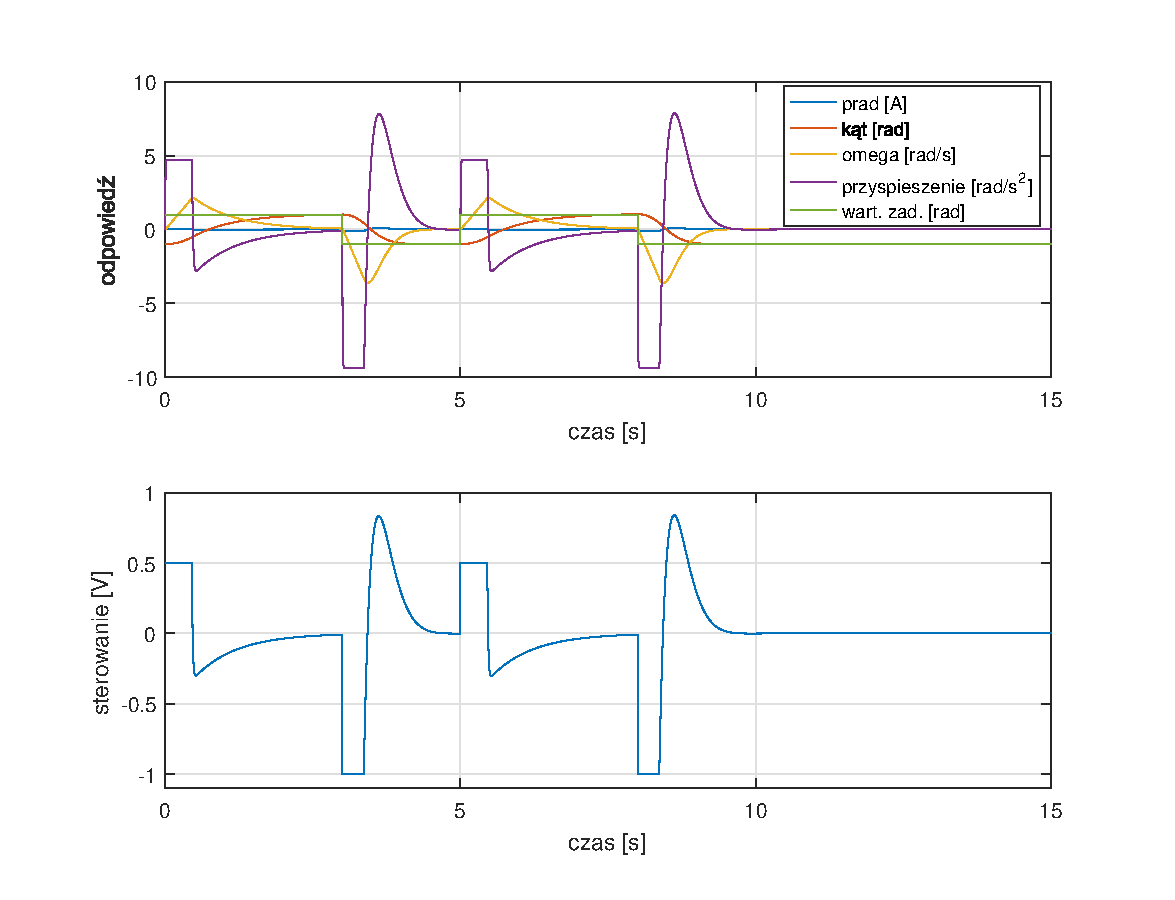
\includegraphics[scale = 0.9]{fig/pid_response.eps}
	\caption		
	{Wartości zmiennych stanu i sterowania.}
	\label{pid_res}
\end{figure} 
	\chapter{Regulator neuronowy}
Regulator neuronowy został zaprojektowany w taki sposób aby otrzymać analogiczne przebiegi sygnałów jak w przypadku klasycznego regulatora PID, wykorzystując do tego celu jeden neuron. Przyjęto, że wektor sygnałów wejściowych będzie miał następującą postać: 
\begin{equation}\label{key}
x = \begin{bmatrix}
\dot {e}\\
e\\
\int e\\
\dfrac{z-z_{min}}{z_{max} - z_{min}}\\
\end{bmatrix}
\end{equation}
gdzie:\\
$e$ - uchyb regulacji\\
$z$ - wartość zadana\\
$z_{min}, \ z_{max}$ - odpowiednio minimalna i maksymalna wartość zadana\\
Z uwagi na fakt, że w rozważanym przypadku wymagane są dwa różne regulatory, współczynnik skalujący zapisano w postaci macierzy: 
\begin{equation}\label{key}
W = \begin{bmatrix}
D_1& P_1& I_1&0\\
D_2& P_2& I_2&0\\
0&0&0&1
\end{bmatrix}
\end{equation} 
Stała składowa dla tak przyjętej postaci regulatora jest trójelementowym wektorem:
\begin{equation}\label{key}
b = \begin{bmatrix}
0\\0\\0
\end{bmatrix}
\end{equation}
Uwzględniając fakt, iż przy przemieszczaniu pustej lub pełnej szklanki należy zmieniać nastawy regulatorów, przyjęto następującą postać funkcji aktywacji:
\begin{equation}\label{key}
f(u,z) = f_{sat1} ((1-z) \cdot u_1 + z \cdot u_2) \cdot (1-z) + f_{sat2} ((1-z) \cdot u_1 + z \cdot u_2) \cdot z
\end{equation}
gdzie: \\
$z - $przeskalowania wartość zadana do przedziału [0,1]\\
$u_1, \ u_2 - $wartości sterowania odpowiednio od regulatorów dla pełnej i pustej szklanki,\\
$f_{sat1}, \ f_{sat2}$ - funkcje saturacji dla pełnej i pustej szklanki.
 \\
\newpage
 Przeanalizowano dwie postaci funkcji saturacji: 
 \begin{enumerate}
 	\item klasyczna funkcja opisana równaniem :
 	\begin{equation}\label{sat_klas}
 	f_{sat}(x) = 
 	\begin{cases}
 	-K       & \quad x < y_{min}\\
 	x  & \quad x \in [y_min, \ y_max]\\
 	K       & \quad x > y_{max}\\
 	\end{cases}
 	\end{equation}
 	\item przybliżenie funkcją sigmoidalną postaci:
 	\begin{equation}\label{key}
 	f_{sat}(x) = (\dfrac{2}{1+\exp{-\beta \cdot x}} - 1) \cdot K
 	\end{equation}
 \end{enumerate}
gdzie:\\
$K$ - maksymalna dozwolona wartość sterowania podawanego na obiekt.\\
Parametry funkcji sigmoidlanych $\beta$ zostały dobrane za pomocą funkcji \textit{fmincon} tak, aby zminimalizować różnice w stosunku do zależności opisanych równaniami \ref{sat_klas}. Finalnie otrzymano następujące wartości parametrów:\\
$\beta1 = -2.65$\\
$\beta2 = -5.33$\\

\begin{figure}[h!]
	\centering
	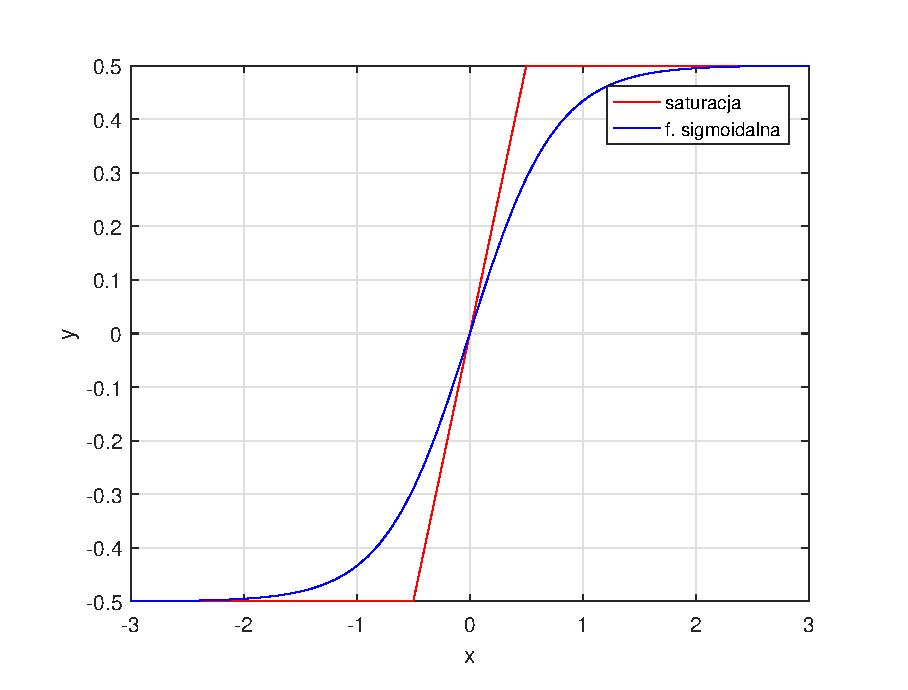
\includegraphics[scale = 0.8]{fig/por_sat_1.eps}
	\caption		
	{Porównanie saturacji i funkcji sigmoidalnej - pełna szklanka.}
	\label{por_sat1}
\end{figure} 

\begin{figure}[h!]
	\centering
	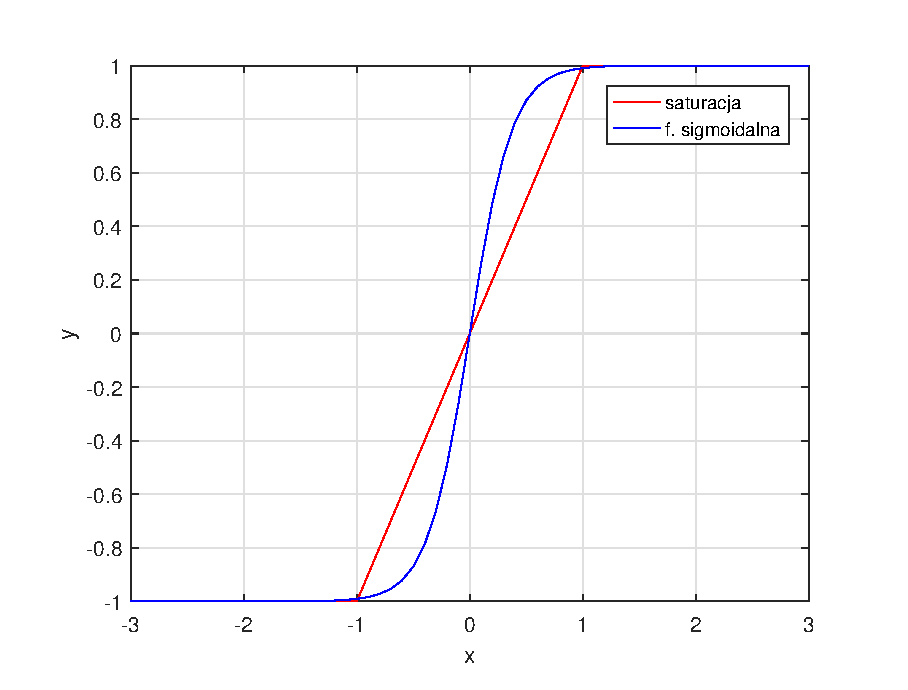
\includegraphics[scale = 0.8]{fig/por_sat_2.eps}
	\caption		
	{Porównanie saturacji i funkcji sigmoidalnej - pusta szklanka.}
	\label{por_sat2}
\end{figure} 

\begin{figure}[h!]
	\centering
	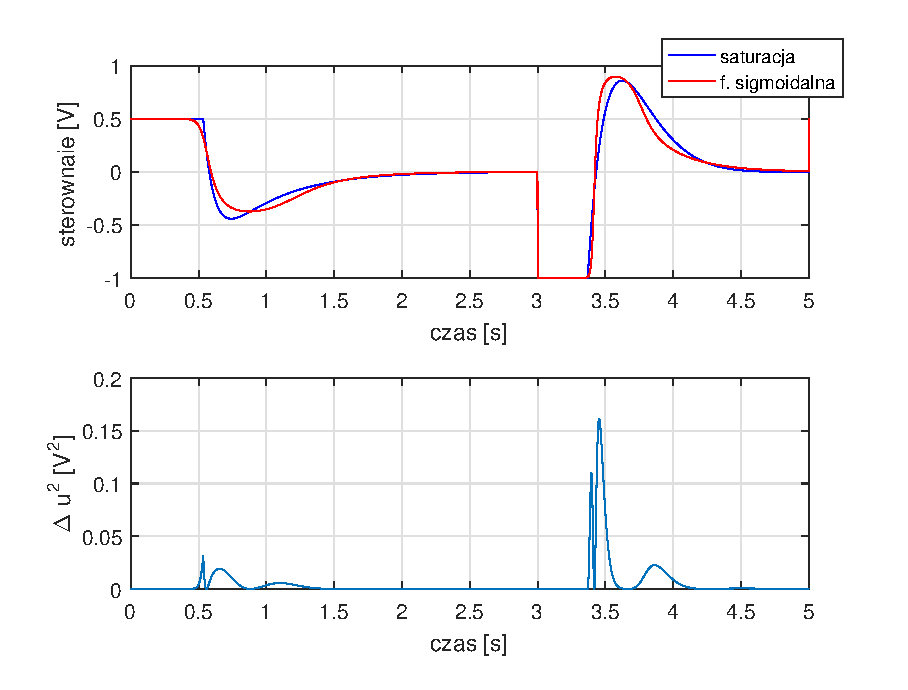
\includegraphics[scale = 1]{fig/por_ster_n.eps}
	\caption		
	{Porównanie sterowania dla regulatora neuronowego.}
	\label{neuron_ster_por}
\end{figure}
\FloatBarrier


\section{Optymalizacja nastaw regulatora}
Wykorzystując funkcję optymalizacyjną środowiska MATLAB, \textit{fmincon},  dobrano nastawy regulatora neuronowego opisanego w poprzedniej części w taki sposób, aby minimalizować wska\'znik jakości $J_3$. 
Poniżej zaprezentowano wartości poszczególnych parametrów regulatora oraz wartości wska\'zników jakości. \\
\\
$J1 = 2.089 \ [rad^2 \cdot s]$\\
$J2 = 0.438 \ [v^2 \cdot s] $\\
$J3 = 2.527$ \\
\\
$W = \begin{bmatrix}
D_1& P_1& I_1&0\\
D_2& P_2& I_2&0\\
0&0&0&1
\end{bmatrix} = 
\begin{bmatrix}
0.2402&2.6707& 1.282&0\\
0.0661& 0.7348&0.3541&0\\
0&0&0&1
\end{bmatrix} 
$
\begin{figure}[h!]
	\centering
	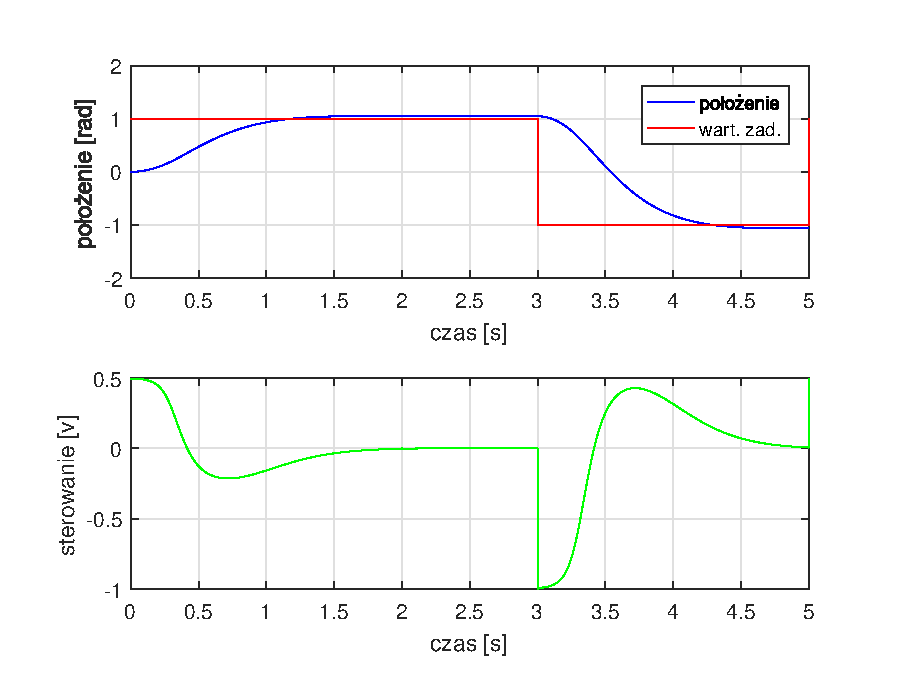
\includegraphics[scale = 1]{fig/neural_opt.eps}
	\caption		
	{Opdowied\'x układu po optymalizacji $J = J_3$.}
	\label{neuron_ster_opt}
\end{figure}
\\
Uwzględniając fakt, że w omawianym układzie saturację zastąpiono funkcją sigmoidalną, w wyniku działania regulatora otrzymano uchyb ustalony. Aby zniwelować ten efekt, zmieniono postać wska\'znika jakości wykorzystywanego w funkcji optymalizującej na :
\begin{equation}\label{key}
J = J_3 + 10 \cdot |z - \alpha_k|
\end{equation}
gdzie:\\
$z - $ wartość zadana,\\
$\alpha_k$ - położenie ramienia w stanie ustalonym.\\\\
Dla tak zmodyfikowanego wska\'znika jakości otrzymano następujące parametry układu regulacji:\\
\\
$J1 = 1.963 \ [rad^2 \cdot s]$\\
$J2 = 0.7543 \ [v^2 \cdot s] $\\
$J3 = 2.718$ \\
\\
$W = \begin{bmatrix}
	D_1& P_1& I_1&0\\
	D_2& P_2& I_2&0\\
	0&0&0&1
	\end{bmatrix} = 
	 \begin{bmatrix}
	 	0.2410&2.9867& 1.5563&0\\
	0.0635& 3.0089&0.9648&0\\
	0&0&0&1
	\end{bmatrix} 
$

\begin{figure}[h!]
	\centering
	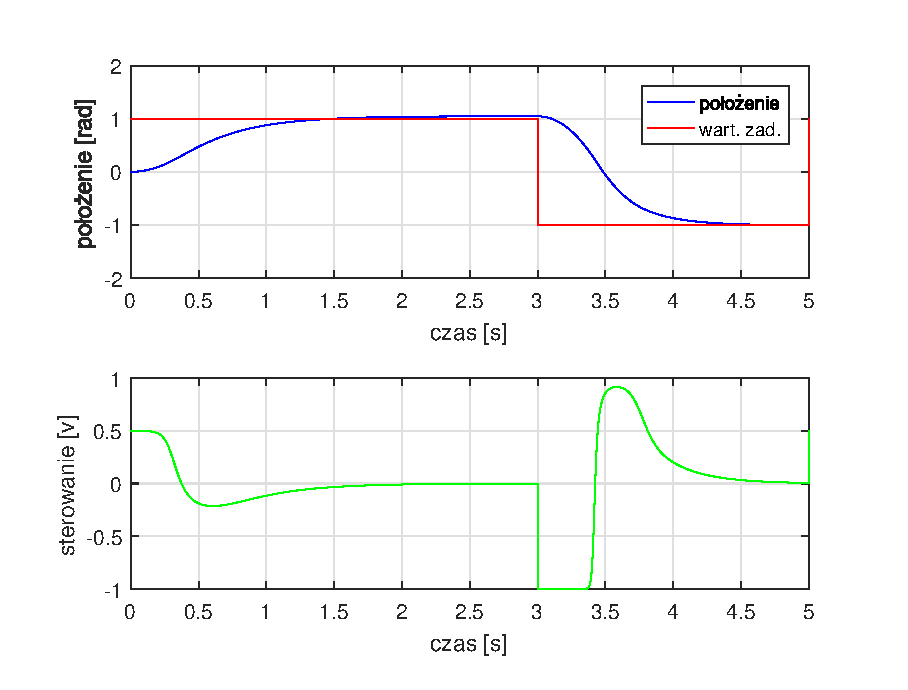
\includegraphics[scale = 1]{fig/neural_opt_uchyb.eps}
	\caption		
	{Opdowied\'x układu po optymalizacji $J = J_3 + |z - \alpha_k|$.}
	\label{neuron_ster_opt_uchyb}
\end{figure}

\FloatBarrier
\newpage
\section{Porównanie wska\'zników jakości}
Poniżej zamieszono porównanie wska\'zników jakości dla trzech różnych regulatorów oraz wartości wspomnianych wska\'zników po przeprowadzonej optymalizacji.

\begin{table}[h]
	\caption{Porównanie wska\'zników jakości regulator PID - neuronowy + saturacja - neuronowy + f. sigmoidalna.}
	\label{por_reg_pid_n_n}
	\centering
	
	\begin{tabular}{|c|M{2.5cm}|M{2.5cm}|M{2.5cm}|}
		\hline
		\multicolumn{1}{|l|}{\begin{tabular}[c]{@{}l@{}}Regulator \textbackslash\\ Wska\'znik jakości\end{tabular}} &$J_1$&$J_2$&$J_3$\\
		\hline
		PID &3.739&   0.841 &  4.580\\
		\hline
		Neuronowy + saturacja &3.739 &  0.841 &  4.580\\
		\hline
		Neuronowy + f. sigmoidalna & 3.741 &  0.857 &  4.597\\
		\hline
		OPTYMALIZACJA\\
		\hline
		Neuronowy1 & 2.08 & 0.438 &  2.527\\
		\hline
		Neuronowy2 & 1.963 &  0.7543 &  2.718\\
		\hline
	\end{tabular}
\end{table}
\FloatBarrier

\section{Projektowanie regulatora neuronowego z użyciem Neural Toolbox.}
	
Zadanie polegało na zbadaniu jaka struktura regulatora neuronowego najlepiej odwzoruje pracę układu z regulatorem PID. Na podstawie sygnału sterującego, wygenerowanego przez zaprojektowany we wcześniejszej części regulator PID, badano, która z rozpatrywanych struktur regulatora jest najlepsza pod względem minimalizacji całki z różnicy pomiędzy sterowaniem referencyjnym i sygnałem pochodzącym z otrzymanego regulatora. Do przeprowadzenia tej części ćwiczenia wykorzystano przybornik Neural Network ze środowiska MATLAB. \\

Rozpatrywano różne postaci sygnałów wejściowych:
\begin{enumerate}
	\item trzy ostatnie wartości uchybu regulacji,
	\item trzy ostatnie wartości uchybu regulacji plus ostatnia wartość referencyjnego sygnału sterującego.
\end{enumerate} 	
Dodatkowo sprawdzono jak liczba neuronów wpływa na wyniki eksperymentu. Rozpatrywano odpowiednio 10 i 20 neuronów w strukturze regulatora.\\
\\
Otrzymane wyniki przedstawione są w tabeli \ref{optNeural}

	\begin{table}[h]
		\caption{Porównanie różnych struktur regulatora neuronowego w stosunku do regulatora PID.}
		\label{optNeural}
		\centering
		
		\begin{tabular}{|c|M{2.5cm}|M{2.5cm}|M{2.5cm}|M{2.5cm}|}
			\hline
			Wska\'znik jakości&10 neuronów&20 neuronów&10 neuronów + sterowanie&20 neuronów + sterowanie\\
			\hline
			e $[V^2 \cdot s]$&11.7862 &   1.5767 &   0.1073& $1.391 \cdot 10^{-5}$ \\
			\hline
		\end{tabular}
	\end{table}
	
	
	\begin{figure}[h!]
		\centering
		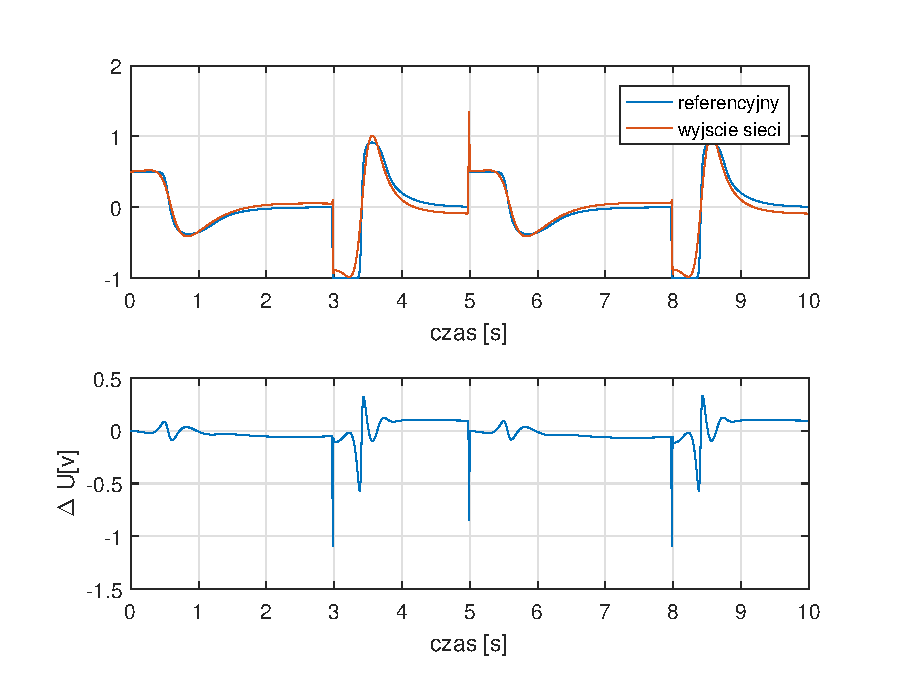
\includegraphics[scale = 0.8]{fig/10neuron.eps}
		\caption		
		{Porównanie sterowania referencyjnego z wyjściem regulatora neuronowego, liczba neuronów = 10.}
		\label{10n}
	\end{figure}

\begin{figure}[h!]
	\centering
	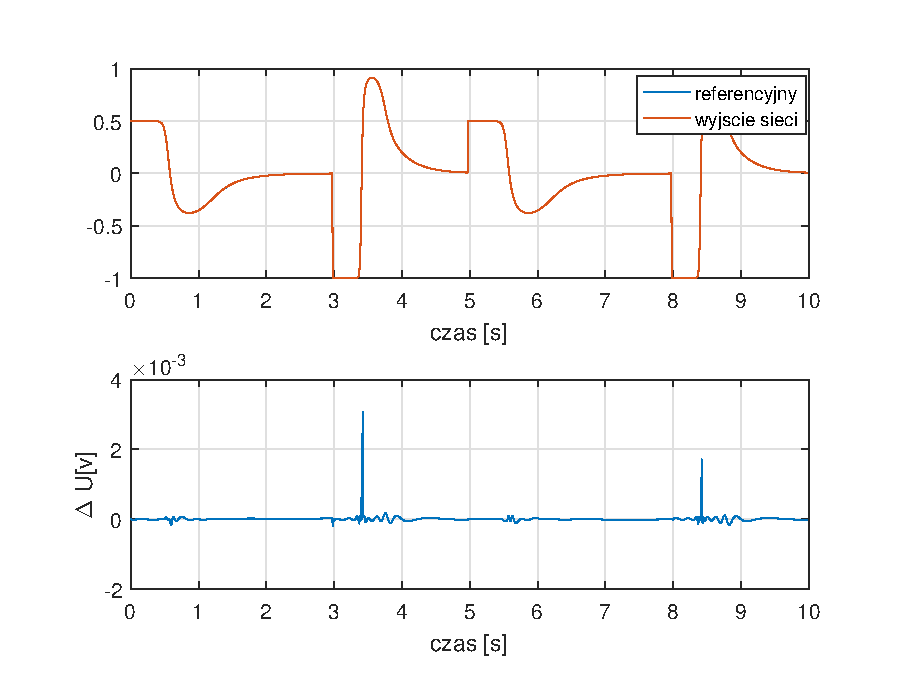
\includegraphics[scale = 0.8]{fig/20neuronU.eps}
	\caption		
	{Porównanie sterowania referencyjnego z wyjściem regulatora neuronowego liczba neuronów = 2.}
	\label{20nU}
\end{figure}

\FloatBarrier
\newpage
	\chapter{Regulator rozmyty}

W tej sekcji przedstawiono wyniki symulacji działania przyjętego układu z regulatorem rozmytym Mamdaniego. Cały proces projektowania struktury regulatora został przeprowadzony w toolbox-ie \textit{Fuzzy} środowiska \textit{Matlab}. Głównym celem przeprowadzonych badań było zapoznanie się z zasadą działania regulatora rozmytego i  jak najlepsze odwzorowanie działania oryginalnego regulatora PID. \\
Zdecydowano, że sygnałami wejściowymi, na których bazował regulator będą uchyb i pochodna uchybu regulacji. Na bazie przebiegów wcześniej wspomnianych sygnałów została zaprojektowana baza reguł. Ze względu na różną dynamikę układu, która zależała od poziomu wypełnienia szklanki, wprowadzono różne reguły dla sterowania. Wszystkie reguły w zależności od wartość uchybu regulacji i jego pochodnej podane są w tabeli \ref{fuzzy_table}. Symbole $P$ i $ P_p$ oznaczają odpowiednio regułę "dodatnią" dla pełnej i pustej szklanki.\\
W ramach przeprowadzonych badań symulacyjnych porównano działania regulatora na bazie wcześniej przyjętych wska\'zników jakości dla różnych postaci funkcji przynależności.

\begin{table}[h]
	\caption{Tabla reguł regulatora fuzzy. $N$ - wart. ujemna, $Z$ - wart. zerowa, $P$ - wart. dodatnia, $P_p$ - wart dodatnia dla pustej szklanki}
	\label{fuzzy_table} 
	\centering
	
	\begin{tabular}{|c|M{2.5cm}|M{2.5cm}|M{2.5cm}|}
		\hline
		$e / \dfrac{de(t)}{dt}$ &$N$&$Z$&$P$\\
		\hline
		$N$ &$Z$& $N$ & $N$\\
		\hline
		$Z$ &$N$& $Z$ & $P$\\
		\hline
		$P$ &$P_p$&  $P_p$ & $Z$\\
		\hline
		
	\end{tabular}
\end{table}
\FloatBarrier
\newpage
\section{Pierwszy zestaw funkcji przynależności}

\begin{figure}[h!]
	\centering
	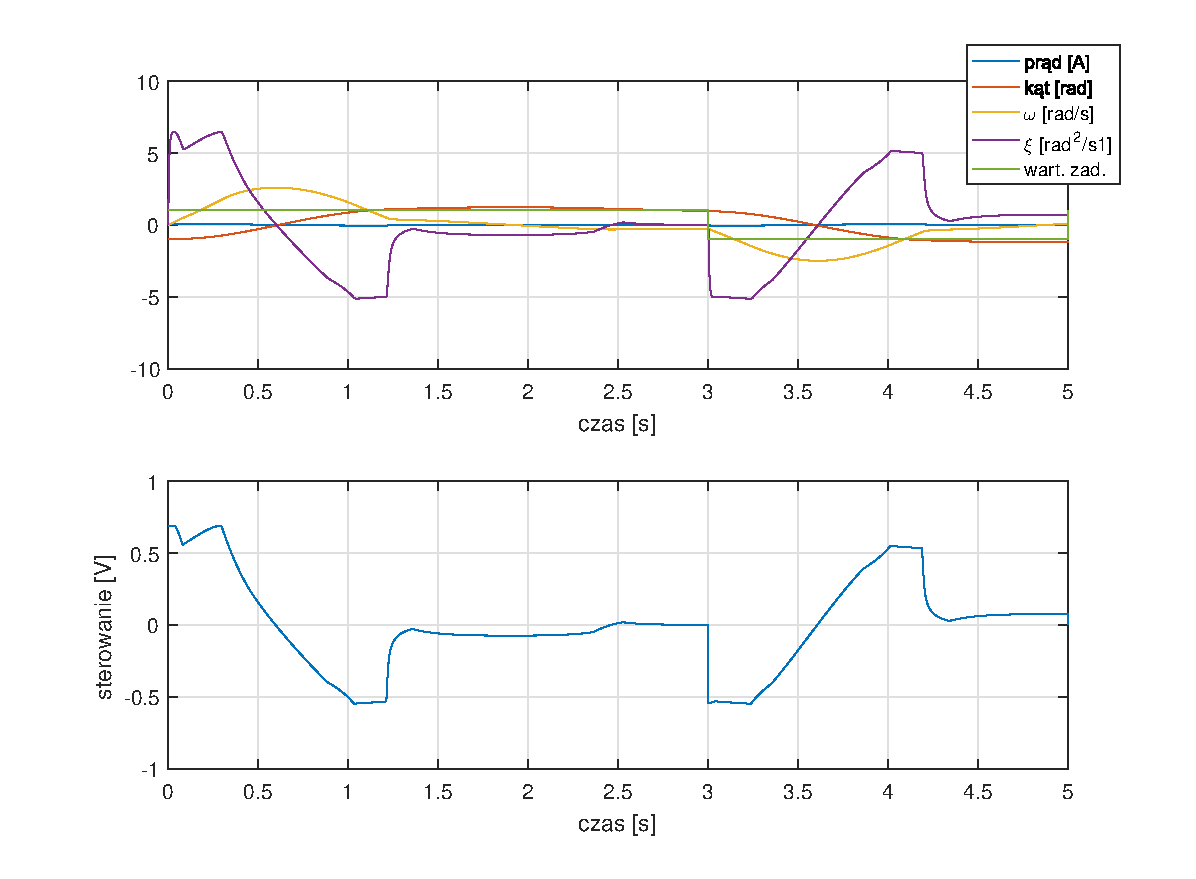
\includegraphics[scale = 0.75]{fig/fuzzy_odp.eps}
	\caption		
	{Odpowied\'z obiektu dla regulatora rozmytego.}
	\label{fuzzyOdp}
\end{figure}

 \begin{figure}[h!]
	\noindent\makebox[\textwidth]{
		\centering
		\subfloat[][Reguły dla uchybu regulacji.]{
			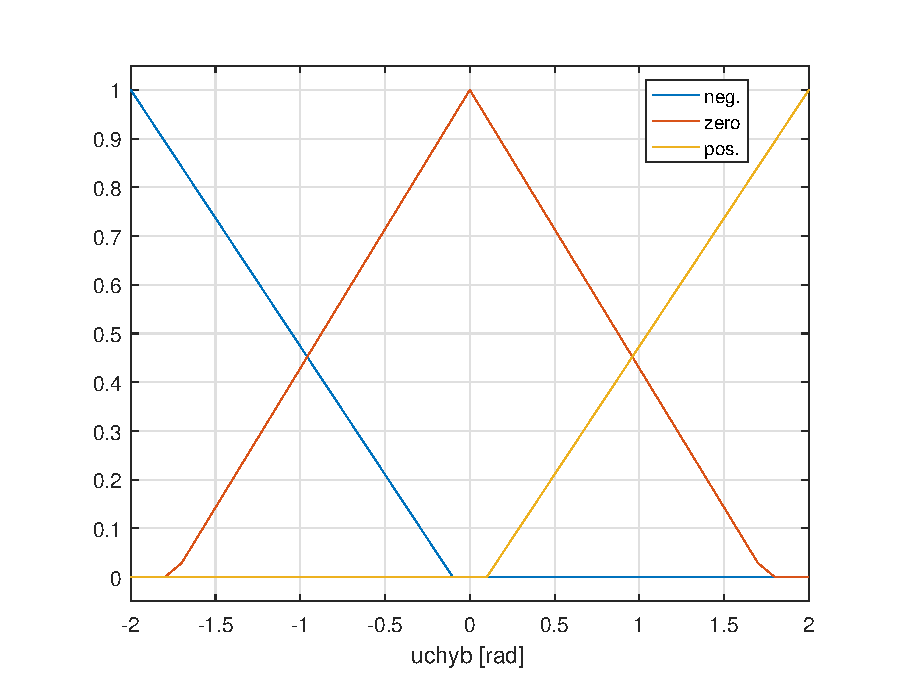
\includegraphics[scale=0.60]{fig/e_rules.eps}
			\label{e_rules1}
		}
		\hfill
		%\begin{figure}[h!]
		%	\centering
		\subfloat[][Reguły dla pochodnej uchybu.]{
			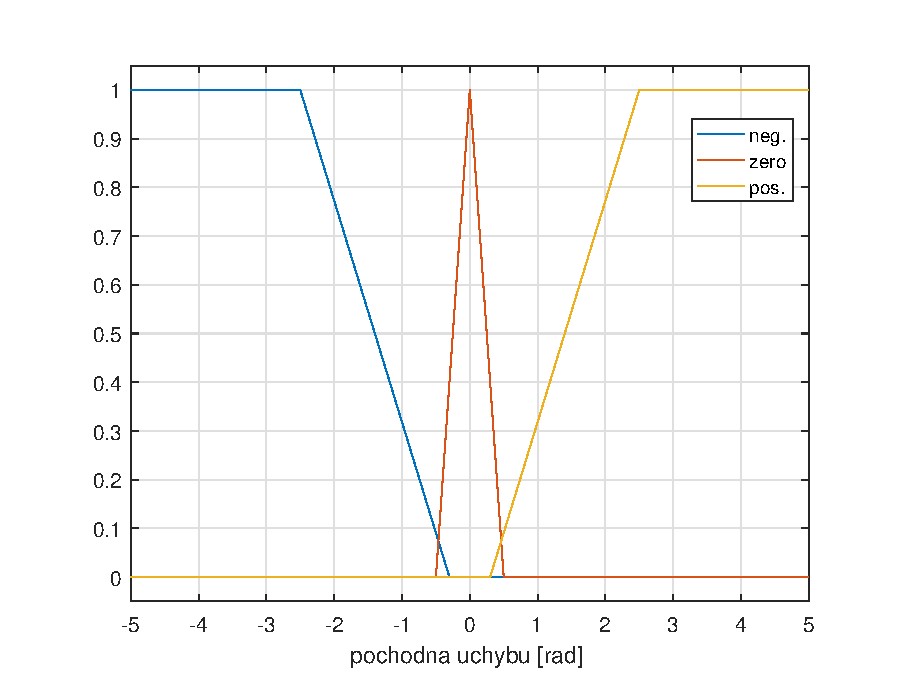
\includegraphics[scale=0.60]{fig/de_rules.eps}
			\label{de_rules1}
		}
		
		%{a) Porównanie wyjścia obiektu i estymaty. b) Porównanie błędów wyjścia i estymaty.}
	}
	\caption{Reguły dla pierwszego zestawu funkcji przynależności.}		
\end{figure}

\begin{figure}[h!]
	\centering
	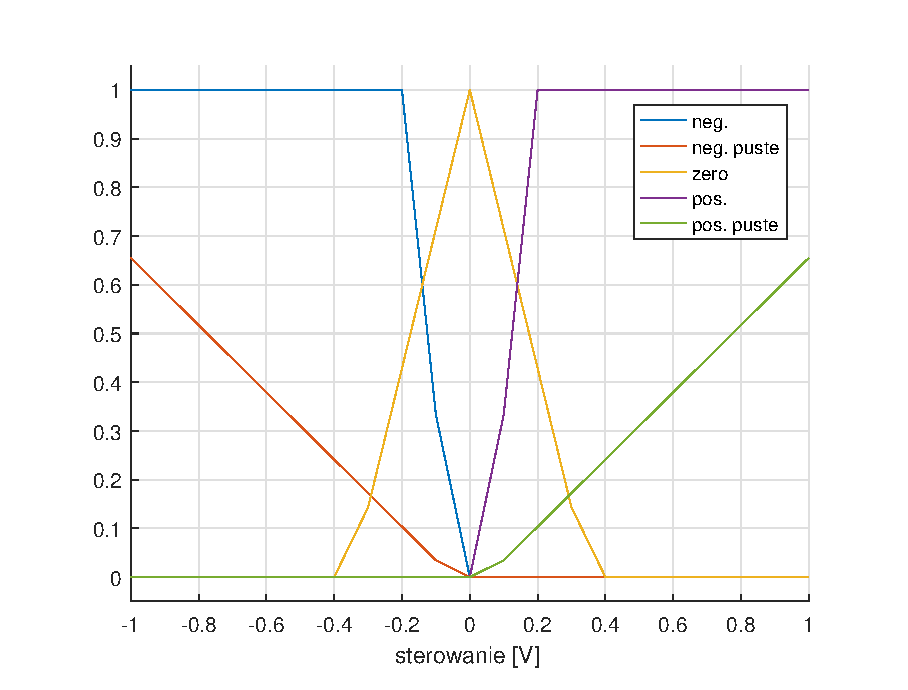
\includegraphics[scale = 0.65]{fig/u_rules.eps}
	\caption		
	{Reguły dla sterowania -  I zestaw funkcji przynależności.}
	\label{u_rules1}
\end{figure}

\FloatBarrier
\section{Drugi zestaw funkcji przynależności}
\label{mamdani2}
Na rysunku \ref{set2_surface} zaprezentowano płaszczyznę wyznaczoną przez przyjęte reguły.
\begin{figure}[h!]
	\centering
	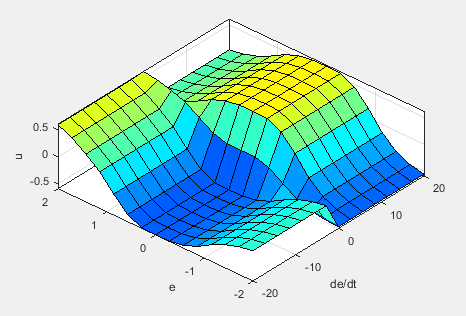
\includegraphics[scale = 0.8]{fig/fuzzySurface.PNG}
	\caption		
	{Płaszczyzna sterowań wyznaczona przez reguły zestawu nr II.}
	\label{set2_surface}
\end{figure}

\begin{figure}[h!]
	\centering
	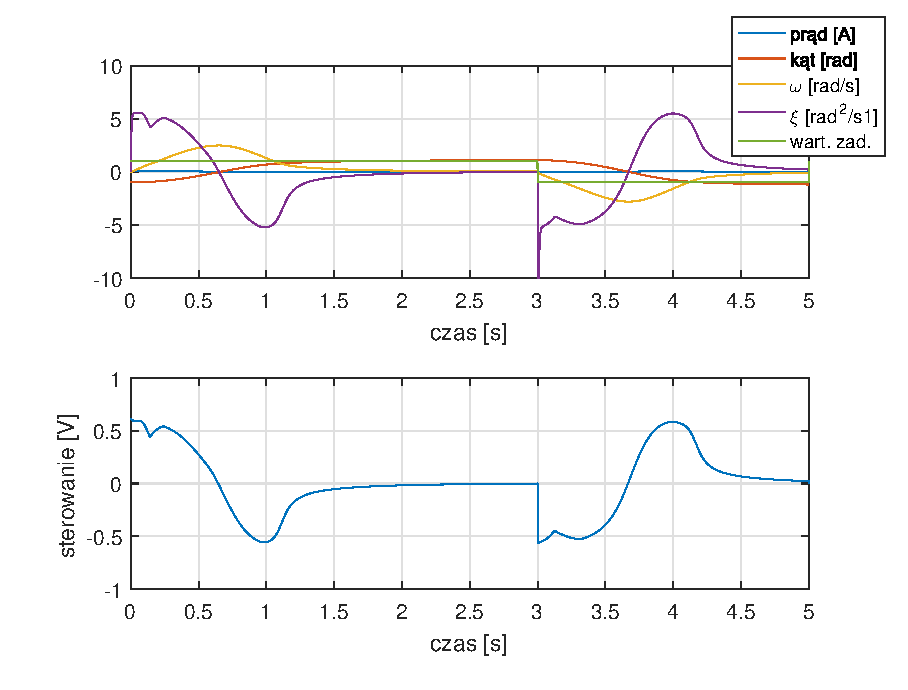
\includegraphics[scale = 1]{fig/fuzzy_odp2.eps}
	\caption		
	{Odpowied\'z obiektu dla regulatora rozmytego, II zestaw funkcji przynależności.}
	\label{fuzzyOdp2}
\end{figure}

 \begin{figure}[h!]
	\noindent\makebox[\textwidth]{
		\centering
		\subfloat[][Reguły dla uchybu regulacji.]{
			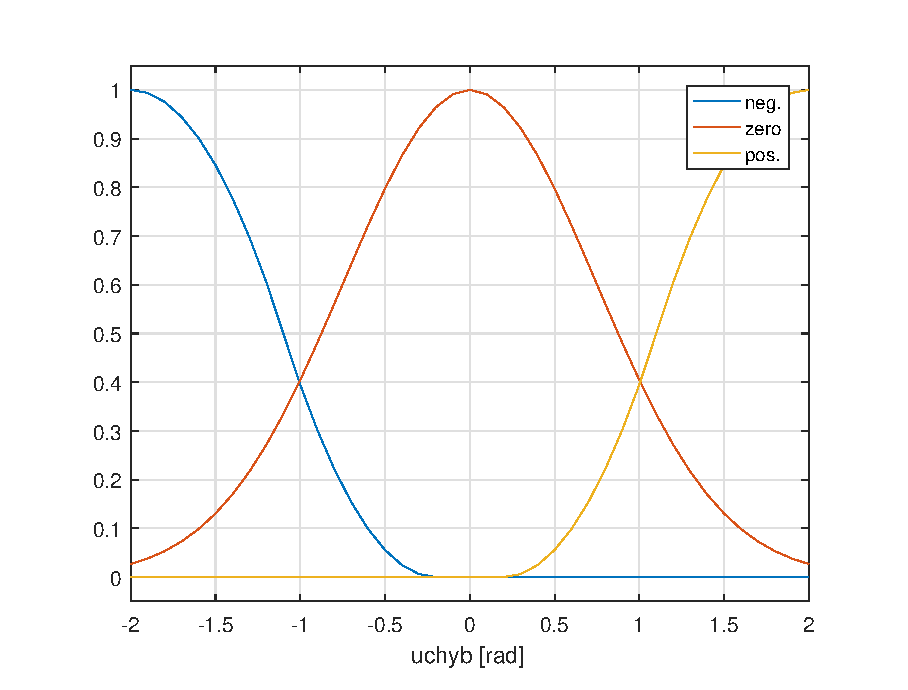
\includegraphics[scale=0.65]{fig/e_rules2.eps}
			\label{e_rules2}
		}
		\hfill
		%\begin{figure}[h!]
		%	\centering
		\subfloat[][Reguły dla pochodnej uchybu.]{
			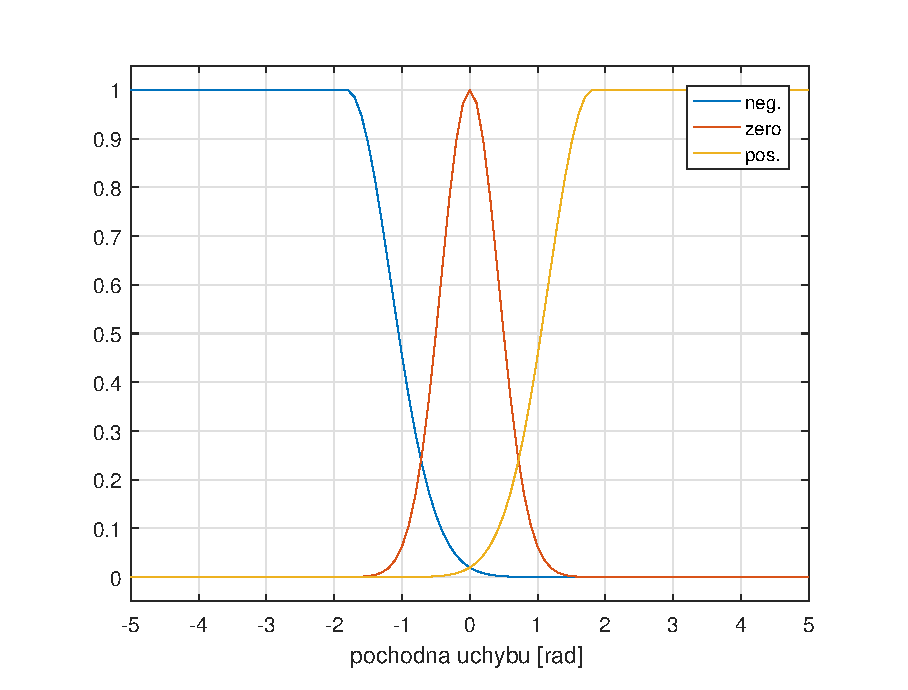
\includegraphics[scale=0.65]{fig/de_rules2.eps}
			\label{de_rules2}
		}
		
		%{a) Porównanie wyjścia obiektu i estymaty. b) Porównanie błędów wyjścia i estymaty.}
	}
	\caption{Reguły dla drugiego zestawu funkcji przynależności.}		
\end{figure}

\begin{figure}[h!]
	\centering
	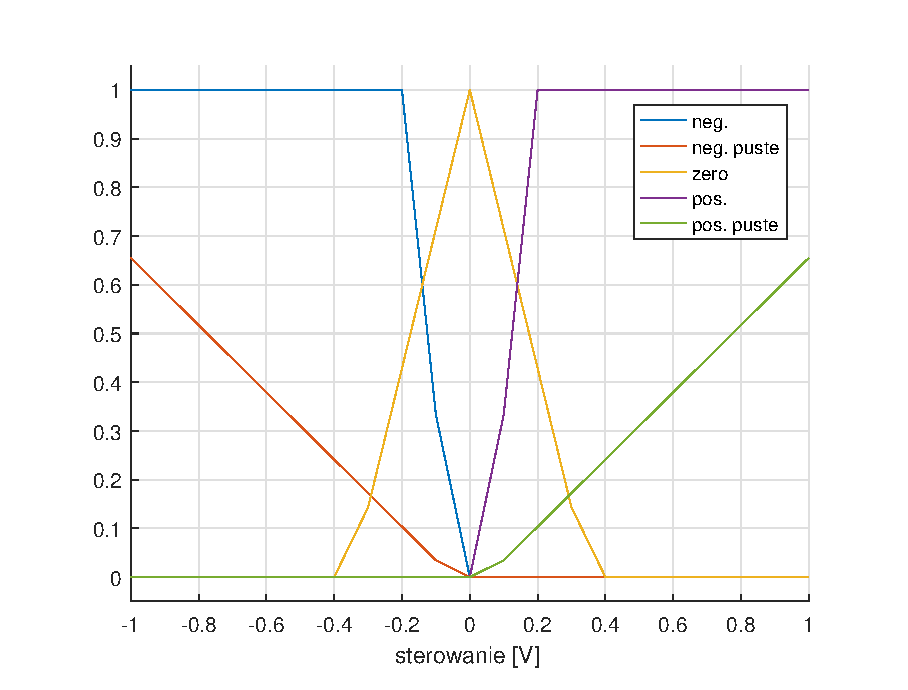
\includegraphics[scale = 0.65]{fig/u_rules.eps}
	\caption		
	{Reguły dla sterowania -  II zestaw funkcji przynależności.}
	\label{u_rules2}
\end{figure}
\FloatBarrier

\section{Porównanie}

Na rysunku \ref{fuzzy_por} przedstawiono porównanie przebiegów odpowiedzi obiektu dla każdego z rozpatrywanych zestawów reguł. W tabeli \ref{fuzzy_wsk} zapisano wartości wska\'zników jakości dla obu rozpatrywanych przypadków.
\begin{figure}[h!]
	\centering
	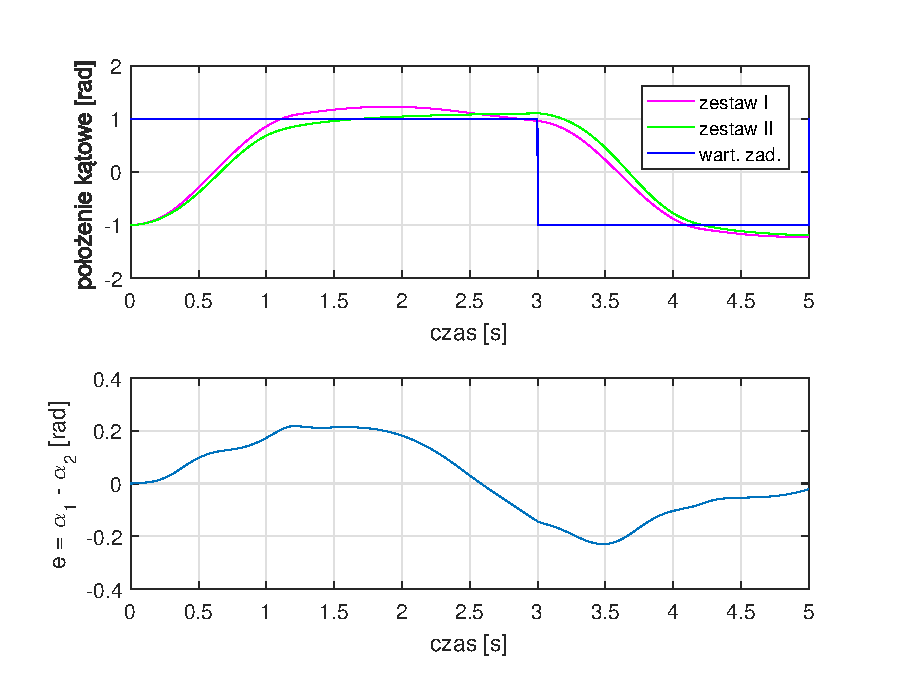
\includegraphics[scale = 1]{fig/por_fuzzy_sets.eps}
	\caption		
	{Porównanie działania regulatora dla oby zestawów reguł.}
	\label{fuzzy_por}
\end{figure}

\begin{table}[h]
	\caption{Wska\'zniki jakości dla regulatora PD - fuzzy.}
	\label{fuzzy_wsk}
	\centering
	
	\begin{tabular}{|c|M{2.5cm}|M{2.5cm}|M{2.5cm}|}
		\hline
		Funkcje przynależności &$J_1$&$J_2$&$J_3$\\
		\hline
		I zestaw &3.624&  1.96 &  5.583\\
		\hline
		II zestaw &4.201&  1.667 &  5.868\\
		\hline
				
	\end{tabular}
\end{table}
\FloatBarrier
Z przebiegów zamieszczonych na rysunku \ref{fuzzy_por} i danych z tabeli \ref{fuzzy_wsk} wynika, że w przypadku drugiego zestawu funkcji przynależności odpowied\'z obiektu ma gorszą dynamikę i mniejsze przeregulowanie niż w przypadku zestawu nr 1. W przypadku wykorzystania funkcji gaussowskich otrzymano dużo lepszy wska\'znik jakości $J_2$, który jest odpowiednikiem energii dostarczonej do układu.

\newpage
\section{Regulator Takagi - Sageno}
Główną różnicą pomiędzy regulatorem rozmytym typu Takagi-Sageno (1985 r.), a strukturą regulatora zaproponowaną przez Mamdaniego jest sposób wyznaczania wartości sygnału wyjściowego. W przypadku regulatora Mamdaniego po przeprowadzeniu fuzyfikacji sygnałów wejściowych następował etap wnioskowania dla każdej z reguł oraz agregacji otrzymanych wartości. Następnie otrzymany zbiór rozmyty był poddawany procesowi defuzyfikacji wykorzystując do tego celu metodę środka ciężkości. W przypadku regulatora Takag-Sageno proces wyliczania sygnału wyjściowego jest mniej skomplikowany. Wyjściowe funkcje przynależności są w tym przypadku stałymi lub funkcjami liniowymi sygnałów wejściowych, a wartość wyjściowa wyliczana jest jako średnia ważona tych wartości.

\subsection{Manualny dobór struktury regulatora}
W rozpatrywanym przypadku reguły przynależności do zbiorów rozmytych dla sygnału wejściowego są identyczne jak te opisane w podrozdziale \ref{mamdani2}. Wielkościami poszukiwanymi w tym przypadku były wartości funkcji wyjściowej dla każdego z rozpatrywanych przypadków. Przyjęto, że będzie ona przyjmować wartości ze zbioru ${-1, 0, 1}$. W tabeli \ref{sagenoRulesTab} zamieszczone są wszystkie reguły zaprojektowanego regulatora.
\begin{table}[h!]
	\caption{Tabelka reguł regulatora typu Takagi-Sageno.}
	\label{sagenoRulesTab}
	\centering
	
	\begin{tabular}{|c|M{2.5cm}|M{2.5cm}|M{2.5cm}|}
		\hline
		$e / \dfrac{de(t)}{dt}$ &$N$&$Z$&$P$\\
		\hline
		$N$ &$0$& $-1$ & $-1$\\
		\hline
		$Z$ &$-1$& $0$ & $1$\\
		\hline
		$P$ &$1$&  $1$ & $0$\\
		\hline
		
	\end{tabular}
\end{table}
\FloatBarrier
%
Jak można zauważyć, tabela \ref{sagenoRulesTab} jest analogiczna do tabeli \ref{fuzzy_table} z tą różnicą, że nieliniowe funkcje przynależności zastąpiono liczbami.\\
Na rysunku \ref{fuzzy_sageno_sufraceMan} zaprezentowano powierzchnię sterowania dla tak dobranej struktury regulatora, a na rysunku \ref{fuzzy_sageno_man} odpowied\'z układu.\\
\begin{figure}[h!]
	\centering
	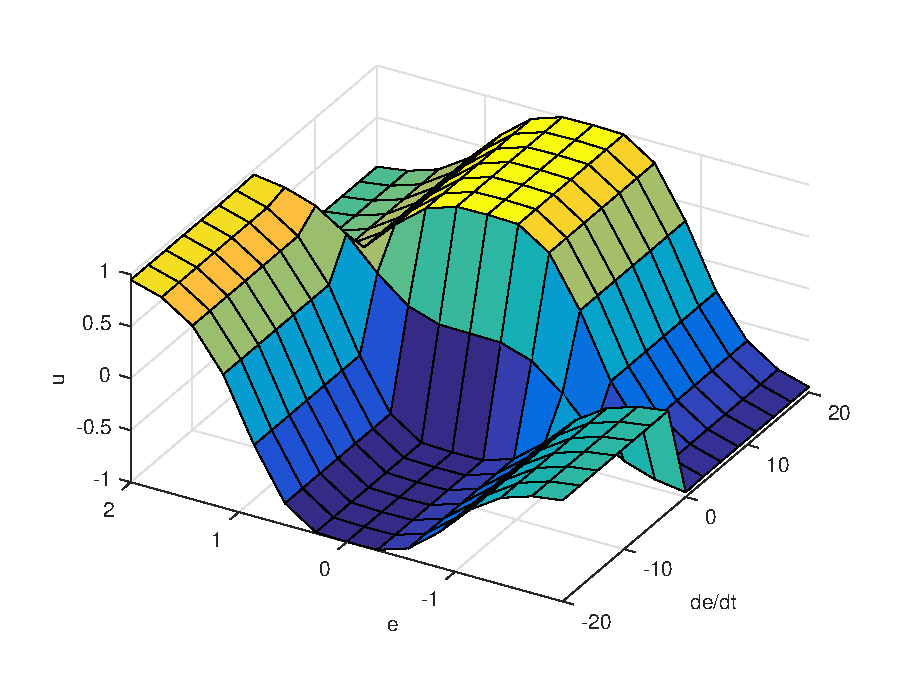
\includegraphics[scale = 0.7]{fig/sagenoManSurface.eps}
	\caption		
	{Powierzchnia sterowania dla regulatora rozmytego typu Takagi-Sageno.}
	\label{fuzzy_sageno_sufraceMan}
\end{figure}

\begin{figure}[h!]
	\centering
	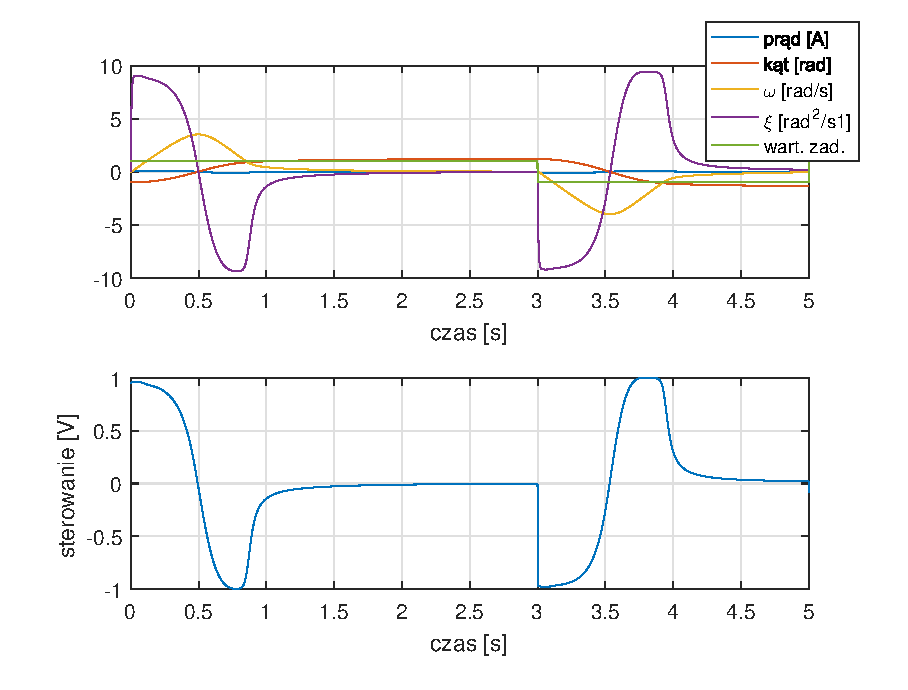
\includegraphics[scale = 0.8]{fig/fuzzy_sagenoMan_odp.eps}
	\caption		
	{Odpowied\'z obiektu dla regulatora rozmytego typu Takagi-Sageno.}
	\label{fuzzy_sageno_man}
\end{figure}
\FloatBarrier
\newpage

\subsection{Optymalizacja struktury regulatora}
W kolejnym kroku wykorzystano funkcję środowiska \textit{Matlab} \textit{genfis1} i \textit{anfis} do wyznaczenia struktury regulatora. W procesie konfiguracji ustawiono gaussowskie funkcje przynależności zarówno dla uchybu regulacji jak i dla jego pochodnej. Na rysunkach \ref{fuzzy_sageno_sufrace} - \ref{fuzzy_sageno_de_rulles} zaprezentowano płaszczyznę sterowania oraz funkcje przynależności zwrócone przez wcześniej wymienione funkcje.
\begin{figure}[h!]
	\centering
	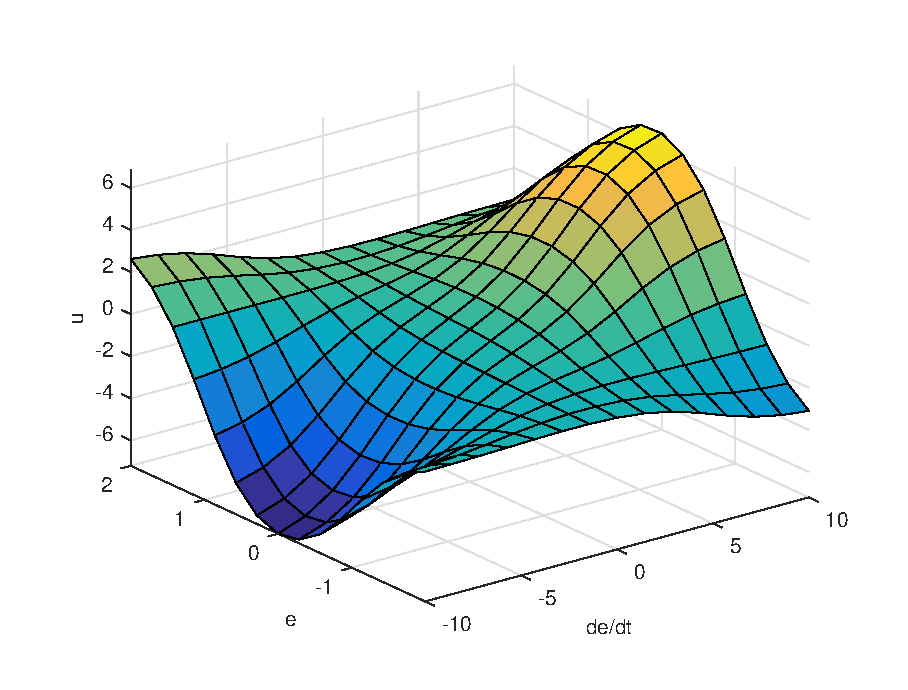
\includegraphics[scale = 0.8]{fig/sagenoOptSurface.eps}
	\caption		
	{Powierzchnia sterowania dla regulatora rozmytego typu Takagi-Sageno po optymalizacji.}
	\label{fuzzy_sageno_sufrace}
\end{figure}

 \begin{figure}[h!]
 	\noindent\makebox[\textwidth]{
	\centering
	\subfloat[][Reguły dla uchybu regulacji.]{
		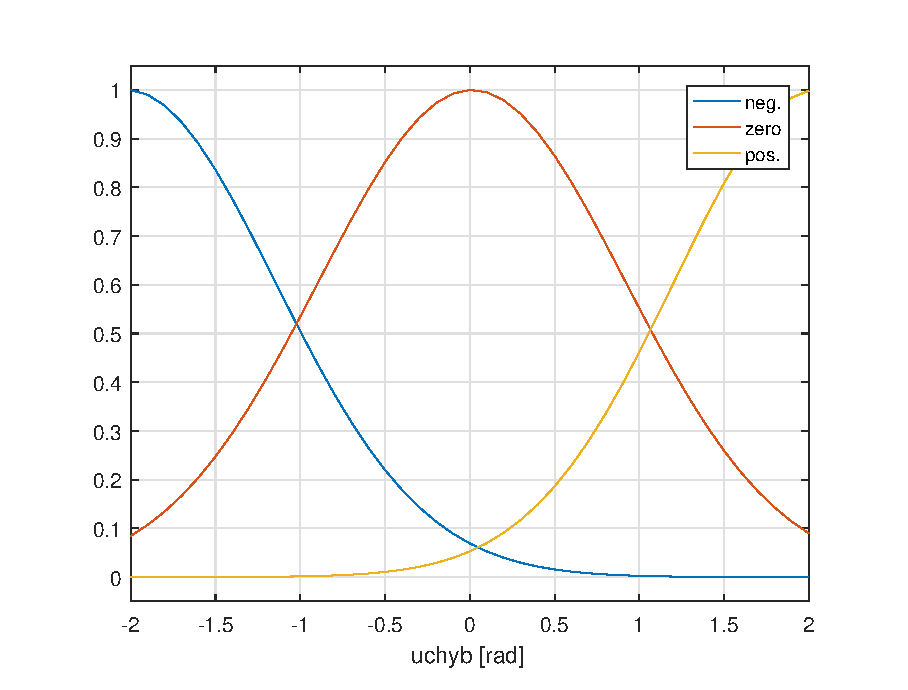
\includegraphics[scale=0.65]{fig/e_rules_sageno.eps}
		\label{fuzzy_sageno_e_rulles}
	}
	\hfill
	%\begin{figure}[h!]
	%	\centering
	\subfloat[][Reguły dla pochodnej uchybu.]{
		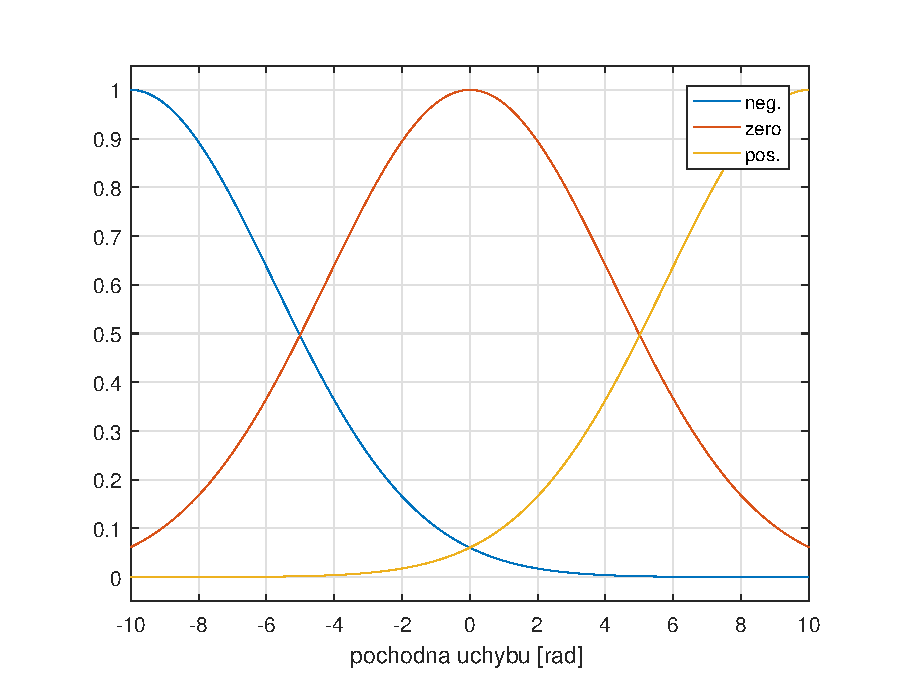
\includegraphics[scale=0.65]{fig/de_rules_sageno.eps}
		\label{fuzzy_sageno_de_rulles}
	}

	%{a) Porównanie wyjścia obiektu i estymaty. b) Porównanie błędów wyjścia i estymaty.}
	}
\caption{Reguły dla regulatora T-S po optymalizacji.}		
\end{figure}

\FloatBarrier
Rysunek \ref{fuzzy_sageno_odp} przedstawia przebiegi wszystkich zmiennych stanu rozważanego układu.
\begin{figure}[h!]
	\centering
	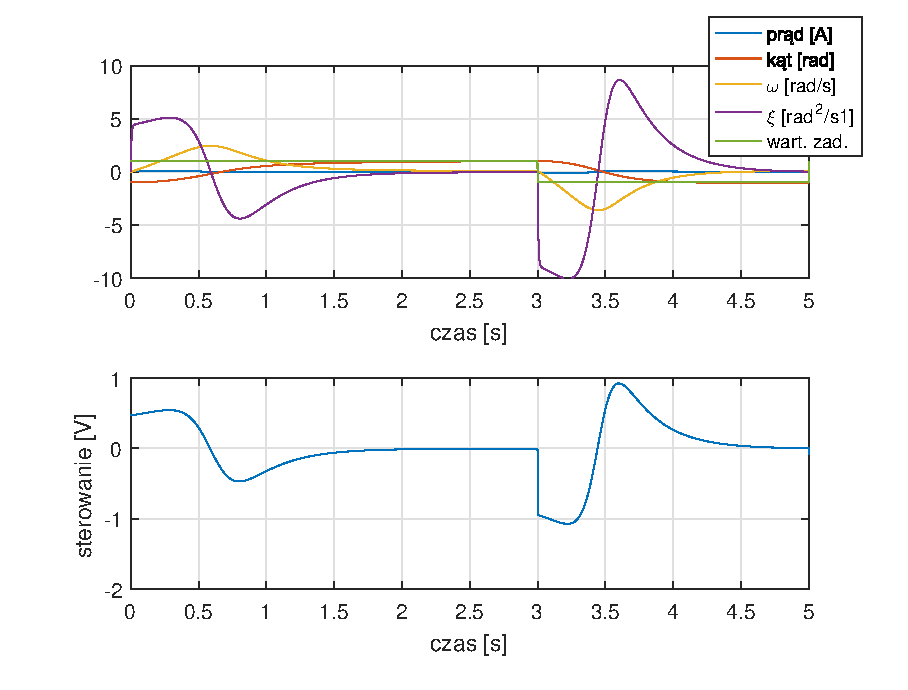
\includegraphics[scale = 1]{fig/fuzzy_sagenoOpt_odp.eps}
	\caption		
	{Odpowied\'z obiektu dla regulatora rozmytego typu Takagi-Sageno po optymalizacji.}
	\label{fuzzy_sageno_odp}
\end{figure}
\FloatBarrier
\newpage
\subsection{Porównanie}

Porównując wartości w tabeli \ref{fuzzy_sageno_wsk} i przebiegi na rysunku \ref{fuzzy_sageno_por} można stwierdzić, że odpowied\'z obiektu dla regulatora otrzymanego w wyniku przeprowadzenia procedury optymalizującej ma gorszą dynamikę niż w przypadku ręcznego strojenia. W zamian za to otrzymaliśmy znacząco lepszą wartość wska\'znika $J_2$ jakości oraz mniejsze przeregulowanie.
\begin{figure}[h!]
	\centering
	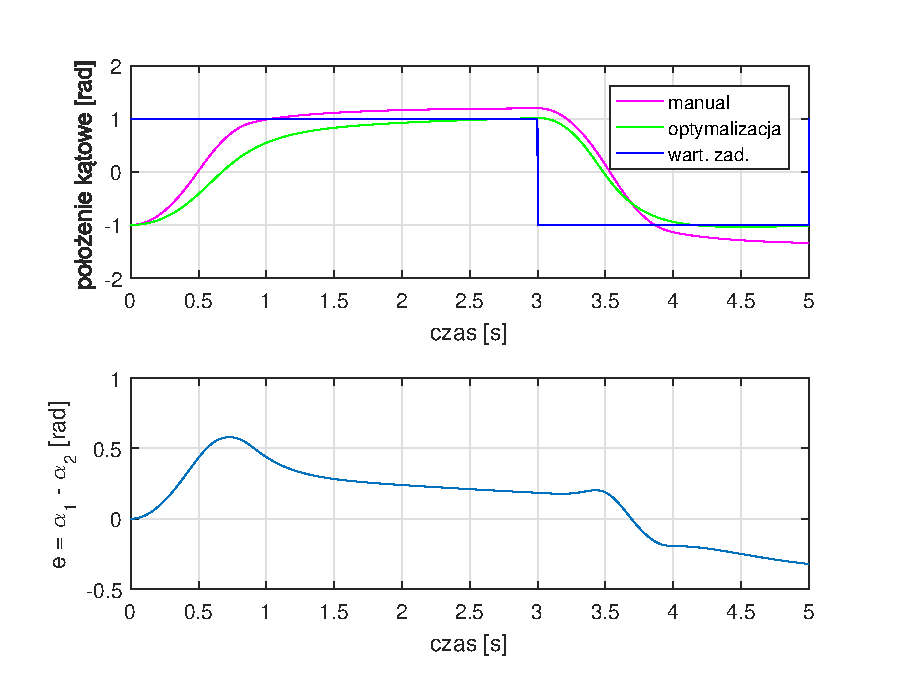
\includegraphics[scale = 0.8]{fig/por_fuzzy_sageno.eps}
	\caption		
	{Porównanie działania regulatora przed i po procesie optymalizacji.}
	\label{fuzzy_sageno_por}
\end{figure}

\begin{table}[h]
	\caption{Porównanie wska\'zników jakości dla regulatora rozmytego typu Takagi-Sageno.}
	\label{fuzzy_sageno_wsk}
	\centering
	
	\begin{tabular}{|c|M{2.5cm}|M{2.5cm}|M{2.5cm}|}
		\hline
		Sposób projektowania &$J_1$&$J_2$&$J_3$\\
		\hline
		manualny &3.497&  2.639 &  6.136\\
		\hline
		optymalizacja &3.642&  0.8707 &  4.513\\
		\hline		
	\end{tabular}
\end{table}
	\chapter{Regulator rozmyty dla modelu helikoptera}
\section{Wstęp}
Celem przedstawionych w niniejszym rozdziale badań było sprawdzenie jak regulator rozmyty współpracuje z rzeczywistym obiektem. Do eksperymentów wykorzystany został model helikoptera oraz jego model matematyczny sporządzony na potrzeby Laboratorium Problemowego. Zadaniem zaprojektowanego regulatora była stabilizacja układu w zadanym położeniu w osi poziomej.

\section{Model matematyczny}
Obiekt opisany jest następującymi równaniami:
\begin{equation}
\begin{aligned}
J_v \frac{d^2\alpha_v}{dt^2} &= -f_v\frac{d\alpha_v}{dt}+a\cdot sin(\alpha_v-\alpha_{v0})+M_v(\omega_v)\\
I_v\frac{d\omega_v}{dt} &= u_v - H_v^{-1}(\omega_v)
\end{aligned}
\label{eq:model_vertical1}
\end{equation}
\noindent gdzie:\newline
\(\alpha_v\) jest kątem obrotu w płaszczyźnie pionowej,\newline
\(J_v\) jest momentem bezwładności względem osi obrotu w płaszczyźnie pionowej,\newline
\(f_v\) jest współczynnikiem tarcia lepkiego,\newline
\(a\) jest momentem sił grawitacji,\newline
\(\alpha_{v0}\) jest kątem równowagi układu w płaszczyźnie pionowej,\newline
\(I_v\) jest momentem bezwładności dużego śmigła,\newline
\(H_v^{-1}(\omega_v)\) jest charakterystyką statyczną układu silnik-śmigło dla silnika głównego,\newline
\(\omega_v\) jest prędkością obrotową silnika głównego,\newline
\(M_v(\omega_v)\) jest momentem sił generowanym przez silnik główny,\newline
\(u_v\) jest współczynnikiem wypełniania sygnału PWM dla silnika głównego.\\\\
%
Równania stanu sporządzone na podstawie równań \ref{eq:model_vertical1} mają postać:
\begin{equation}
\begin{aligned}
\dot x_1 &= x_2\\
\dot x_2 &= -\frac{f_v}{J_v}x_2+\frac{a}{J_v}\sin (\alpha_v-\alpha_{v0})+\frac{M_v(\omega_v)}{J_v}\\
\dot x_3 &= \frac{u_v}{I_v}-\frac{H_v^{-1}(\omega_v)}{I_v}
\end{aligned}
\label{eq:ss_vertical1}
\end{equation}
%
Proces identyfikacji parametrów równań \ref{eq:ss_vertical1} opisany jest w pracy \cite{LP}.

\section{Regulator referencyjny}
Aby dobrać strukturę regulatora rozmytego typu Sageno podjęto decyzję o wykorzystaniu regulatora LQI. Podejście to wymagało zlinearyzowania równań \ref{eq:ss_vertical1} oraz zaprojektowania obserwatora Luengergera (\cite{LP}) w celu estymacji pełnego stanu obiektu.\\ 
Zlinearyzowany model w położeniu poziomym opisany jest równaniem 
\begin{equation}\label{key}
\begin{aligned}
\dot x = Ax + B \\
y = Cx + D
\end{aligned}
\end{equation}
gdzie:
\begin{equation}
\begin{aligned}
A &=
\begin{bmatrix}
0 & 1 & 0\\
-4.4005 & -0.0695 & 0.0244\\
0 & 0 & -2.8870
\end{bmatrix}\\
B &=
\begin{bmatrix}
0\\
0\\
577.5771
\end{bmatrix}\\
C &=
\begin{bmatrix}
1 & 0 & 0
\end{bmatrix}\\
D &= 0
\end{aligned}
\end{equation} 
Przyjęto następujące wartości własne obserwatora:
\begin{equation}
\begin{aligned}
\lambda_1 &= -3\\
\lambda_2 &= -6\\
\lambda_3 &= -9
\end{aligned}
\end{equation}
Obserwator Luenbergera pełnego rzędu opisany jest równaniem różniczkowym
\begin{equation}
\dot w = Aw+L(y-Cw)+Bu
\end{equation}
\noindent gdzie:\newline
\(A\) jest macierzą stanu obserwowanego układu,\newline
\(B\) jest macierzą sterowania obserwowanego układu,\newline
\(C\) jest macierzą wyjścia obserwowanego układu,\newline
\(G\) jest macierzą wybraną tak, by wartości własne macierzy \(A-LC\) miały ujemne części rzeczywiste,\newline
\(w\) estymuje obserwowany stan.
\paragraph*{}
Wybrana macierz \(L\) miała następującą postać:
\begin{equation}
L =
\begin{bmatrix}
15.0434\\
49.9218\\
87.9693
\end{bmatrix}
\end{equation}
%
Regulator LQI opisany jest zależnością 
\begin{equation}
\begin{aligned}
J&=\int\limits_0^{\infty}(x^TQx+u^TRu)dt\\
Q&=\begin{bmatrix}
10 & 0 & 0 & 0\\
0 & 0 & 0 & 0\\
0 & 0 & 0 & 0\\
0 & 0 & 0 & 1
\end{bmatrix}\\
R&=1
\end{aligned}
\end{equation}
\noindent gdzie:\newline
\(x_4\) jest całką z uchybu kąta.\\\\
%
Wektor wzmocnień \ref{wzmocnienieLQI} regulatora został wyliczony za pomocą funkcji \textit{lqi} środowiska \textit{Matlab}.
\begin{equation}
K=\begin{bmatrix}
0.3154 & 0.7105 & 0.0042 & -1
\end{bmatrix}
\label{wzmocnienieLQI}
\end{equation}

\section{Regulator rozmyty}
Do doboru struktury regulatora rozmytego typu Sageno wykorzystano funkcję\textit{genfis} środowiska \textit{Matlab}. W pierwszym etapie sprawdzono jakość regulacji projektując regulator \textit{fuzzy} na bazie modelu matematycznego. Na rysunku  \ref{por_model_lqi_fuzzy} przedstawiono odpowiedzi modelu obiektu w przypadku działania regulatora LQI i fuzzy.\\
%
\begin{table}[h]
	\caption{Porównanie wska\'zników jakości regulator LQI i fuzzy dla modelu.}
	\label{por_reg_lqi_fuzz_model}
	\centering
	
	\begin{tabular}{|c|M{2.5cm}|M{2.5cm}|M{2.5cm}|}
		\hline
		Regulator &$J_1$\\
		\hline
		LQI &0.102\\
		\hline
		fuzzy & 0.102\\
		\hline
	\end{tabular}
\end{table}
\FloatBarrier
Wartości wska\'zników jakości zaprezentowane w tabeli \ref{por_reg_lqi_fuzz_model} oraz przebiegi zaprezentowane na rysunkach \ref{por_model_lqi_fuzzy} i \ref{diff_model_lqi_fuzzy} pokazują że w przypadku matematycznego modelu rozważanego obiektu klasyczny regulator LQI może być z powodzeniem zastąpiony regulatorem rozmytym bez pogorszenia jakości sterowania.

 \begin{figure}[h!]
	\noindent\makebox[\textwidth]{
		\centering
		\subfloat[][Porównanie działania regulatora LQI i fuzzy.]{
			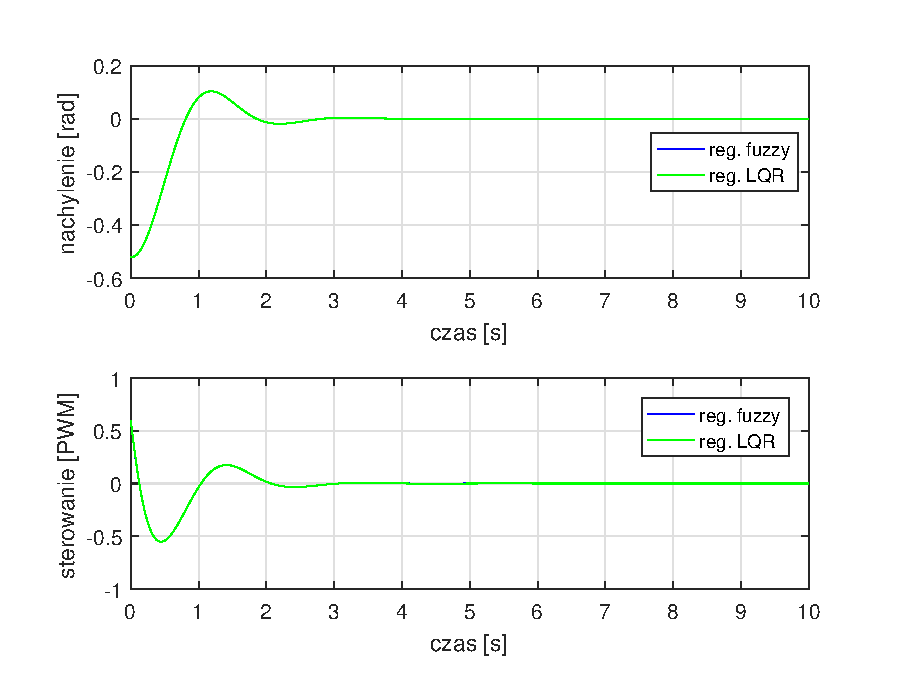
\includegraphics[scale=0.65]{fig/por_fuzzy_model_lqi.eps}
			\label{por_model_lqi_fuzzy}
		}
		\hfill
		%\begin{figure}[h!]
		%	\centering
		\subfloat[][Różnica działania regulatora LQI i fuzzy.]{
			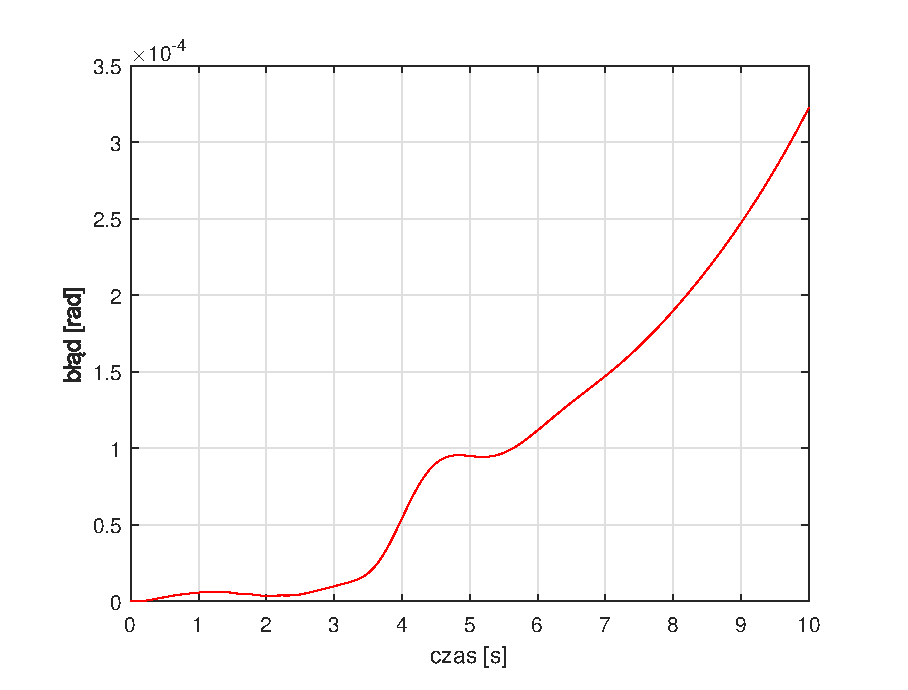
\includegraphics[scale=0.65]{fig/diff_fuzzy_model_lqi.eps}
			\label{diff_model_lqi_fuzzy}
		}
		
		%{a) Porównanie wyjścia obiektu i estymaty. b) Porównanie błędów wyjścia i estymaty.}
	}
	\caption{Działanie regulatora dla modelu obiektu.}		
\end{figure}


%\begin{figure}[h!]
%	\centering
%	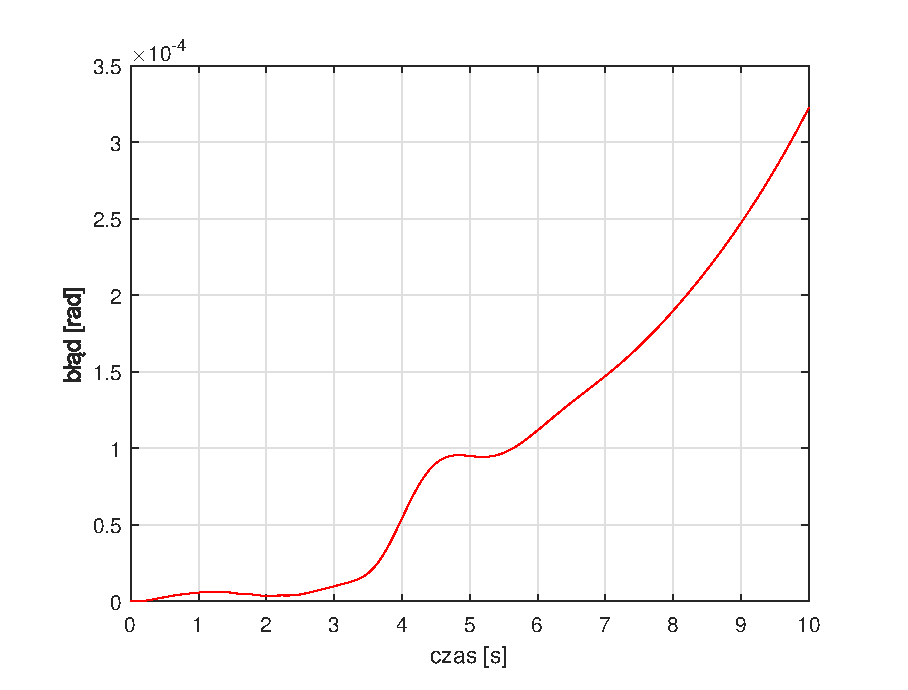
\includegraphics[scale = 0.8]{fig/diff_fuzzy_model_lqi}
%	\caption		
%	{Różnica działania regulatora LQI i fuzzy.}
%	\label{diff_model_lqi_fuzzy}
%\end{figure} 

\begin{figure}[h!]
	\centering
	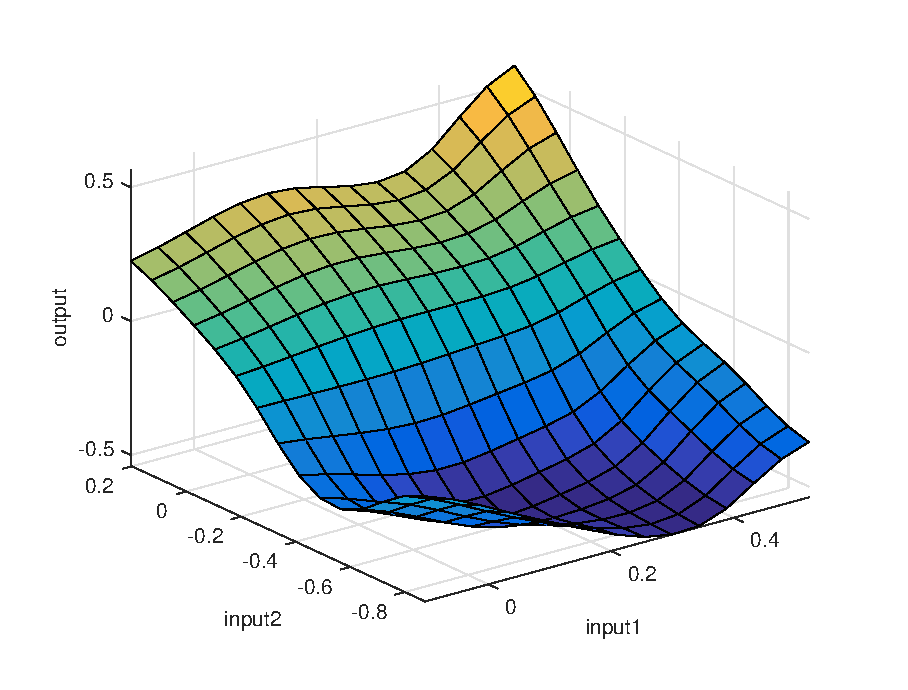
\includegraphics[scale = 0.8]{fig/fuzzy_hel_model_surf.eps}
	\caption		
	{Powierzchnia sterowania dla modelu obiektu rzutowana na pierwszą i drugą zmienną stanu.}
	\label{fuzzy_hel_model_surf}
\end{figure} 
\FloatBarrier
Następnie postanowiono sprawdzić działanie regulatora na rzeczywistym obiekcie. W tym celu na wejście obiektu podano sygnał pokazany na rysunku \ref{stan_obiekt}. Podczas działania układu rejestrowano wartości zmiennych stanu (wyjście z obserwatora Luenbergera), całki uchybu regulacji oraz sterowania.\\
Zdecydowano, że do procedury \textit{genfis} podane zostaną przebiegi zarejestrowanych zmiennych pomiędzy 20 a 40 sekundą. Decyzja ta wynikała z chęci uniknięcia optymalizacji struktury regulatora na danych z początkowego etapu działania obserwatora gdy estymowane wartości zmiennych stanu znacznie odbiegały od rzeczywistych. \\
Niestety nie udało się przetestować działania tak zaprojektowanego regulatora na obiekcie ponieważ \textit{Simulink} nie potrafił uruchomić modelu w czasie rzeczywistym gdy był wykorzystywany w nim bloczek  \textit{Fuzzy Logic Controller}. \\
 \begin{figure}[h]
	\noindent\makebox[\textwidth]{
		\centering
		\subfloat[][Przebieg zmiennych stanu.]{
			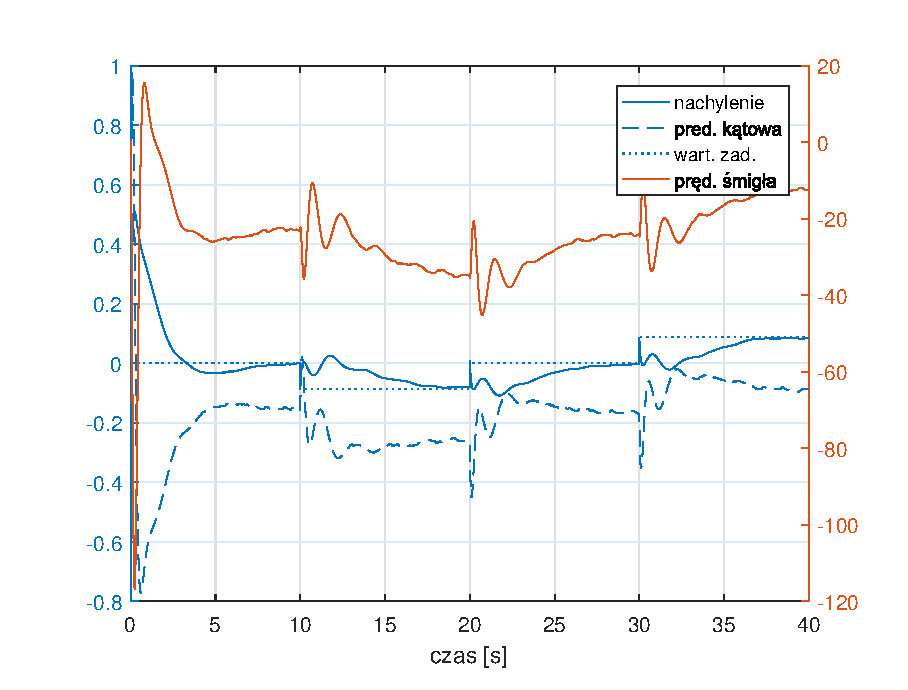
\includegraphics[scale=0.65]{fig/stan_obiekt.eps}
			\label{stan_obiekt}
		}
		\hfill
		%\begin{figure}[h!]
		%	\centering
		\subfloat[][Sterowanie podawane na obiekt.]{
			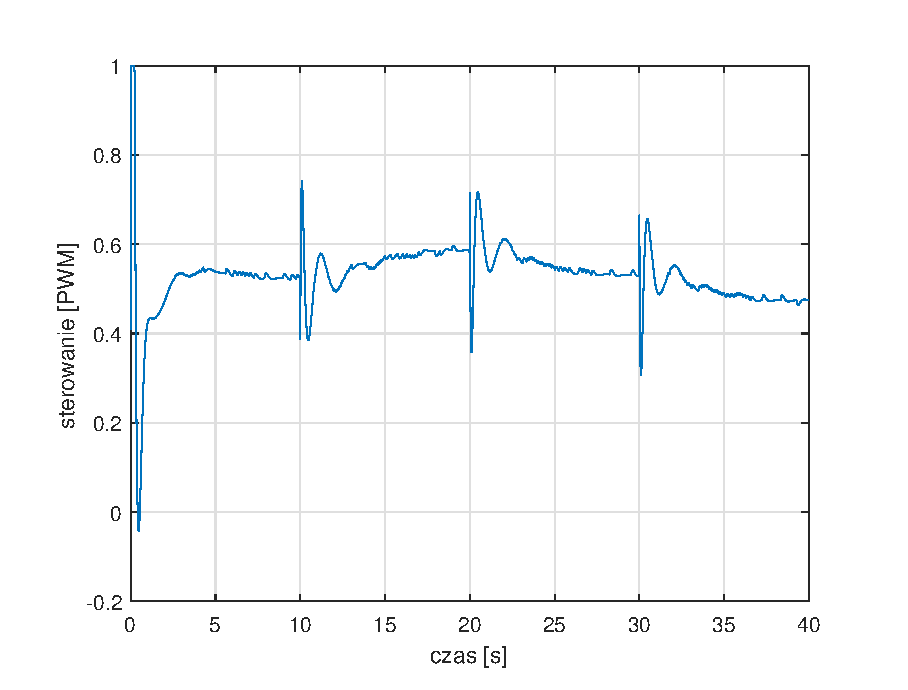
\includegraphics[scale=0.65]{fig/ster_obiekt.eps}
			\label{ster_obiekt}
		}
		
		%{a) Porównanie wyjścia obiektu i estymaty. b) Porównanie błędów wyjścia i estymaty.}
	}
	\caption{Dane wykorzystane do optymalizacji struktury reg. rozmytego.}		
\end{figure}
%
\begin{figure}[h]
	\centering
	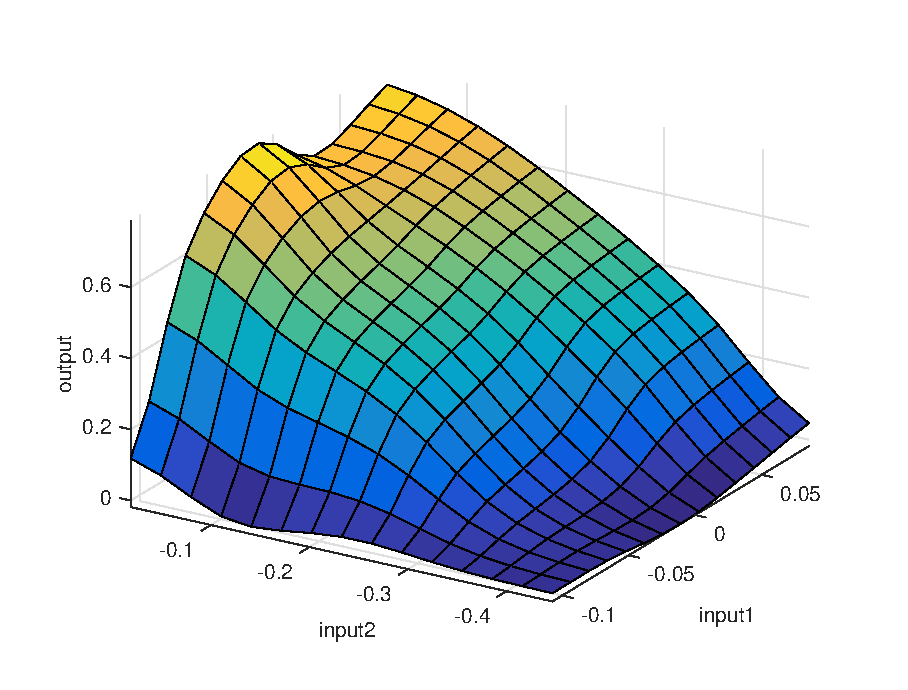
\includegraphics[scale = 0.8]{fig/fuzzy_obiekt_surf.eps}
	\caption		
	{Powierzchnia sterowania dla obiektu rzutowana na pierwszą i drugą zmienną stanu.}
	\label{fuzzy_hel_obiekt_surf}
\end{figure} 
\begin{figure}[h]
	\centering
	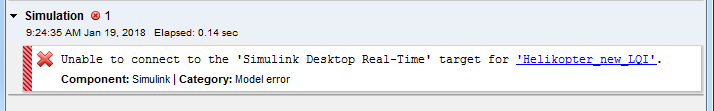
\includegraphics[scale = 0.8]{fig/bladSim.PNG}
	\caption		
	{Błąd zwracany przez \textit{Simulink}.}
	\label{bladSim}
\end{figure} 
\FloatBarrier
 Na podstawie powierzchni sterowania zaprezentowanej na rysunku \ref{fuzzy_hel_obiekt_surf} można stwierdzić że struktura regulatora jest podobna do struktury uzyskanej na podstawie danych symulacyjnych (rysunek \ref{fuzzy_hel_model_surf}). 
 
	\chapter{Wnioski}
Przeprowadzenie badań opisanych w niniejszym sprawozdaniu pozwoliło zapoznać się, z innymi niż dotychczas poznane, rodzajami regulatorów. Zaprojektowanie od podstaw regulatora neuronowego jak i również rozmytego pozwoliło lepiej zrozumieć zasadę ich działania. Dzięki wybraniu, na potrzeby symulacji, prostego obiektu drugiego rzędu mogliśmy w łatwy sposób badać wpływ wprowadzanych w strukturze regulatora modyfikacji na działanie całego systemu. Zamieszczone w sprawozdaniu porównania klasycznych regulatorów z regulatorem neuronowym oraz rozmytym pokazało, że każde z rozważanych podejść daje porównywalne wyniki i może być zastosowane w praktyce. \\
Podsumowując, regulator neuronowy jak i rozmyty spełnił swoją rolę, jednak aby uzyskać zbliżone wyniki do regulatorów klasycznych należało poświęcić więcej czasu na dobraniu odpowiedniej struktury i parametrów regulatora. Wykorzystanie sieci neuronowych bąd\'z też logiki rozmytej może mieć swoje uzasadnienie w przypadku bardziej złożonych systemów. Dla prostych obiektów pierwszego i drugiego rzędu może być ciężko uzyskać lepszą jakość regulacji niż w przypadku regulator PID lub LQ bez wykorzystania dedykowanych narzędzi \textit{Matlab-a}.
	
	\begin{thebibliography}{}
	
	%przykład 
	
	\bibitem{LP}Cebula M., Kowalczyk M., Rubak D.: 
	\emph{Model helikoptera. Laboratorium Problemowe 2}, Kraków 2018
	

	
\end{thebibliography}
	
\end{document}